\documentclass[aspectratio=169]{beamer}
\usetheme{Madrid}
\usepackage[utf8]{vietnam}
\usepackage[vietnamese]{babel}
\usepackage{tasks, fdsymbol}
\usepackage{tikz}
\usepackage{tikz,tkz-tab}
\usepackage{graphicx} 
\usepackage{listings}
\usepackage{pgfplots}
\usepackage{xcolor}
\usepackage{multicol}
\usepackage{blindtext}
\usepackage{tikz}
\usepackage{diagbox}
\usepackage[T1]{fontenc}

\usepackage{amsmath}
\usepackage{amssymb}
\usepackage{color}
\usepackage{xstring}

\definecolor{dkgreen}{rgb}{0,0.6,0}
\definecolor{gray}{rgb}{0.5,0.5,0.5}
\definecolor{mauve}{rgb}{0.58,0,0.82}

\input{listings-python.prf}
\lstset{frame=tb,
  language=C++,
  aboveskip=3mm,
  belowskip=3mm,
  showstringspaces=false,
  columns=flexible,
  basicstyle={\small\ttfamily},
  numbers=none,
  numberstyle=\tiny\color{gray},
  keywordstyle=\color{blue},
  commentstyle=\color{dkgreen},
  stringstyle=\color{mauve},
  breaklines=true,
  breakatwhitespace=true,
  tabsize=3
}

\title{
MỘT SỐ PHƯƠNG PHÁP BẤT ĐẲNG THỨC\\ HÀM LỒI VÀ BẤT ĐẲNG THỨC JENSEN}
\author{\textbf{ NHÓM 6}} 
\date{09/07/2024}
\begin{document}
\titlepage
% 1.1 Sử dụng định nghĩa và biến đổi tương đương
\begin{frame}{
1.1 SỬ DỤNG ĐỊNH NGHĨA \\ VÀ BIẾN ĐỔI TƯƠNG ĐƯƠNG \hspace{3cm}  65.Phạm Phương Thảo} 
%\framesubtitle{} 
\begin{block}{Thứ tự trên tập hợp số thực}
\pause
Trên tập số thực, với hai số $a$ và $b$ có ba trường hợp sau:

\begin{itemize}
    \item Số $a$ bằng số $b$, kí hiệu $a=b$;
    \item Số $a$ lớn hơn số $b$, kí hiệu $a>b$;
    \item Số $a$ nhỏ hơn số $b$, kí hiệu $a<b$.
\end{itemize}
\end{block} 
\pause
Số $a$ lớn hơn hoặc bằng số $b$, tức là $a>b$ hoặc $a=b$, kí hiệu $a\geq b$.

Số $a$ nhỏ hơn hoặc bằng số $b$, tức là $a<b$ hoặc $a=b$, kí hiệu $a\leq b$.
\end{frame}

\begin{frame}{
1.1 SỬ DỤNG ĐỊNH NGHĨA \\ VÀ BIẾN ĐỔI TƯƠNG ĐƯƠNG \hspace{3cm}  65.Phạm Phương Thảo} 
%\framesubtitle{} 
\begin{block}{Khái niệm bất đẳng thức}
\pause
Ta gọi hệ thức dạng $a>b$ (hay $a<0, a\geq b, a\leq b$) là bất đẳng thức và gọi $a$ là vế trái, $b$ là vế phải của bất đẳng thức.
\end{block} 
\pause
Ví dụ: 
\begin{itemize}
    \item $0<1$;
    \item $x>0$;
    \item $\dfrac{a}{b}+\dfrac{b}{a}\geq 2, \forall a,b \in \mathbb{R}^+$.
\end{itemize}
\pause
Chú ý:
\begin{itemize}
    \item Hai bất đẳng thức $1<2$ và $-3<-2$ được gọi là \textit{hai bất đẳng thức cùng chiều};
    \item Hai bất đẳng thức $1<2$ và $-2>-3$ được gọi là \textit{hai bất đẳng thức ngược chiều}.
\end{itemize}
\end{frame} 

\begin{frame}{1.1 SỬ DỤNG ĐỊNH NGHĨA \\ VÀ BIẾN ĐỔI TƯƠNG ĐƯƠNG \hspace{3cm}  65.Phạm Phương Thảo}
\begin{block}{Tính chất}
Nếu $a<b$ và $b<c$ thì $a<c$ (tính chất bắc cầu của bất đẳng thức).
\end{block}
\pause
Chú ý:
Tương tự, các thứ tự lớn hơn ($>$), lớn hơn hoặc bằng ($\geq$), nhỏ hơn hoặc bằng ($\leq$) cũng có tính chất bắc cầu.
\end{frame}

\begin{frame}{1.1 SỬ DỤNG ĐỊNH NGHĨA \\ VÀ BIẾN ĐỔI TƯƠNG ĐƯƠNG \hspace{3cm}  65.Phạm Phương Thảo}
\begin{block}{Liên hệ giữa thứ tự và phép cộng}
\pause
Khi cộng cùng một số vào hai vế của một bất đẳng thức ta được bất đẳng thức mới \textit{cùng chiều} với bất đẳng thức đã cho. 
\end{block} 
\pause
Với ba số $a, b, c$, ta có:
\begin{itemize}
    \item Nếu $a<b$ thì $a+c<b+c$;
    \item Nếu $a\leq b$ thì $a+c \leq b+c$;
    \item Nếu $a>b$ thì $a+c>b+c$;
    \item Nếu $a\geq b$ thì $a+c\geq b+c$.
\end{itemize}
\end{frame}

\begin{frame}{1.1 SỬ DỤNG ĐỊNH NGHĨA \\ VÀ BIẾN ĐỔI TƯƠNG ĐƯƠNG \hspace{3cm}  65.Phạm Phương Thảo}
\begin{block}{Liên hệ giữa thứ tự và phép nhân}
\begin{itemize}
    \item Khi nhân cả hai vế của một bất đẳng thức với cùng một \textit{số dương} ta được bất đẳng thức mới \textit{cùng chiều} với bất đẳng thức đã cho; 
\end{itemize}
\end{block}
\pause
Với ba số $a, b, c$ và $c>0$, ta có:
\begin{itemize}
    \item Nếu $a<b$ thì $ac<bc$;
    \item Nếu $a\leq b$ thì $ac \leq bc$;
    \item Nếu $a>b$ thì $ac>bc$;
    \item Nếu $a\geq b$ thì $ac\geq bc$.
\end{itemize}
\end{frame}

\begin{frame}{1.1 SỬ DỤNG ĐỊNH NGHĨA \\ VÀ BIẾN ĐỔI TƯƠNG ĐƯƠNG \hspace{3cm}  65.Phạm Phương Thảo}
\begin{block}{Liên hệ giữa thứ tự và phép nhân}
\begin{itemize}
    \item Khi nhân cả hai vế của một bất đẳng thức với cùng một \textit{số âm} ta được bất đẳng thức mới \textit{ngược chiều} với bất đẳng thức đã cho; 
\end{itemize}
\end{block}
\pause
Với ba số $a, b, c$ và $c<0$, ta có:
\begin{itemize}
    \item Nếu $a<b$ thì $ac>bc$;
    \item Nếu $a\leq b$ thì $ac \geq bc$;
    \item Nếu $a>b$ thì $ac<bc$;
    \item Nếu $a\geq b$ thì $ac\leq bc$.
\end{itemize}
\end{frame}

\begin{frame}{1.1 SỬ DỤNG ĐỊNH NGHĨA \\ VÀ BIẾN ĐỔI TƯƠNG ĐƯƠNG \hspace{3cm}  65.Phạm Phương Thảo}
\begin{block}{Ví dụ 0.}
Cho ba số thực $a, b, c$. Chứng minh rằng: $$a^2+b^2+c^2 \geq ab+bc+ca.$$
\end{block}
\pause
Ta có:
$a^2+b^2+c^2 \geq ab+bc+ca.$

$\Leftrightarrow a^2+b^2+c^2-ab-bc-ca \geq 0.$

\pause
$\Leftrightarrow 2a^2+2b^2+2c^2-2ab-2bc-2ca \geq 0.$
\pause

$\Leftrightarrow (a^2-2ab+b^2)+(b^2-2bc+c^2)+(c^2-2ca+a^2) \geq 0.$

$\Leftrightarrow (a-b)^2+(b-c)^2+(c-a)^2 \geq 0.$

\pause
Bất đẳng thức luôn đúng do đó ta có được điều phải chứng minh.

Dấu "$=$" xảy ra khi và chỉ khi $a=b=c$.
\end{frame}

\begin{frame}{1.1 SỬ DỤNG ĐỊNH NGHĨA \\ VÀ BIẾN ĐỔI TƯƠNG ĐƯƠNG \hspace{3cm}  65.Phạm Phương Thảo}
\begin{block}{Ví dụ 1.}
Cho ba số thực $a, b, c$. Chứng minh rằng: $$3(a^2+b^2+c^2) \geq (a+b+c)^2 \geq 3(ab+bc+ca).$$
\end{block}
\pause
Ta có: $3(ab+bc+ca).$

\pause

$=ab+bc+ca+2(ab+bc+ca).$

\pause
$\leq a^2+b^2+c^2+2(ab+bc+ca).$

$=(a+b+c)^2.$

\pause
$\leq a^2+b^2+c^2+2(a^2+b^2+c^2).$

$=3(a^2+b^2+c^2).$

Ta được điều phải chứng minh.

Dấu "$=$" xảy ra khi và chỉ khi $a=b=c$.
\end{frame}

\begin{frame}{1.1 SỬ DỤNG ĐỊNH NGHĨA \\ VÀ BIẾN ĐỔI TƯƠNG ĐƯƠNG \hspace{3cm}  65.Phạm Phương Thảo}
\begin{block}{Bài 1.}
Cho ba số thực dương $x, y, z$ sao cho $x+y+z=1$. Chứng minh rằng:
$$\sqrt{6x+1}+\sqrt{6y+1}+\sqrt{6z+1}\leq 3\sqrt{3}.$$
    
\end{block}
\pause
Đặt $a=\sqrt{6x+1}; b=\sqrt{6y+1}; c=\sqrt{6z+1}$; $a, b, c>0$.

\pause
Khi đó, ta có:

$a^2+b^2+c^2=6x+1+6y+1+6z+1=6(x+y+z)+3=6.1+3=9$.

\pause
Ta cần chứng minh: $a+b+c\leq 3\sqrt{3}$.

\pause
Sử dụng kết quả ở \textbf{Ví dụ 1.} Ta có:

$3(a^2+b^2+c^2) \geq (a+b+c)^2.$
\pause

$\Leftrightarrow 3.9 \geq (a+b+c)^2.$ 

Mà $a, b, c>0$ nên ta có: $3\sqrt{3}\geq a+b+c$.
\end{frame}

% 1.2 SỬ dụng tam thức bậc hai

\begin{frame}{1.2 SỬ DỤNG TAM THỨC BẬC HAI \hspace{3cm}  66. Đặng Hồng Thái} 
     \begin{block}{Định lí về dấu của tam thức bậc hai}
            \pause
        Xét $f(x)=ax^2+bx+c  (a\ne 0)$ \\  \pause
        \vspace{0,4cm}
        $f(x)=a\left(x^2+\dfrac{b}{a}.x+\dfrac{c}{a}\right)$ 
        $=a\left(x^2+2.x.\dfrac{b}{2a}+\dfrac{b^2}{4a^2}-\dfrac{b^2}{4a^2}+\dfrac{c}{a}\right)$ \pause
        $=a\left[\left(x+\dfrac{b}{2a}\right)^2-\dfrac{b^2-4ac}{4a^2}\right]$  \\
        \vspace{0,4cm} \pause
        $f(x)=a\left[\left(x+\dfrac{b}{2a}\right)^2-\dfrac{\Delta}{4a^2}\right]$ \\
        \pause
        \begin{center}
             \begin{tabular}{|c|c|c|}
             \hline
             & $a>0$ & $a<0$  \\
             \hline
             $\Delta<0$ & $f(x)>0$ & $f(x)<0$ \\  
             \hline
             \pause
             $\Delta = 0$ & $f(x) \geq 0$ & $f(x) \leq 0$ \\ 
             \hline
             \pause
             $\Delta>0$ & $f(x)=0$ có hai nghiệm $x_1<x_2$ & $f(x)=0$ có hai nghiệm $x_1<x_2$ \\
             \hline
            \end{tabular}
        \end{center}
    \end{block}
\end{frame}


\begin{frame}{1.2 SỬ DỤNG TAM THỨC BẬC HAI \hspace{3cm}  66. Đặng Hồng Thái} 
%\framesubtitle{} 
    \begin{block}{Định lí về dấu của tam thức bậc hai}
        \textbf{Định lí 1.}  $f(x)>0$ với mọi $x$ khi và chỉ khi 
                $\begin{cases}
		 	a>0 \\
		 	\Delta <0
		 	\end{cases}$    \\
         \textbf{Định lí 2.}  $f(x)\geq0$ với mọi $x$ khi và chỉ khi 
                $\begin{cases}
		 	a>0 \\
		 	\Delta \leq0
		 	\end{cases}$    \\
         \textbf{Định lí 3.}  $f(x)<0$ với mọi $x$ khi và chỉ khi 
                $\begin{cases}
		 	a<0 \\
		 	\Delta <0
		 	\end{cases}$    \\
         \textbf{Định lí 4.}  $f(x)\leq0$ với mọi $x$ khi và chỉ khi 
                $\begin{cases}
		 	a<0 \\
		 	\Delta \leq0
		 	\end{cases}$ \\
         \textbf{Định lí 5.}  $f(x)=0$ có nghiệm $x_1<x_2$ khi và chỉ khi           $\Delta\geq 0$. Khi đó \\
                \hspace{2cm} $f(x) = a(x-x_1)(x-x_2) \text{và} \begin{cases}
		 	x_1+x_2=-\dfrac{b}{a} \\
		 	x_1x_2=\dfrac{c}{a}
		 	\end{cases}$
    \end{block} 
\end{frame}


\begin{frame}{1.2 SỬ DỤNG TAM THỨC BẬC HAI \hspace{3cm}  66. Đặng Hồng Thái} 
%\framesubtitle{} 
    \begin{block}{Ví dụ 1}
        Cho $a,b$ là các số thực bất kì. Chứng minh rằng:
        \begin{center}
            $x^2y^4+2(x^2+2)y^2+4xy+x^2\geq4xy^3$
        \end{center}
    \end{block} 
    \begin{center}
        \textbf{Lời giải:}
    \end{center}
    \pause
        Bất đẳng thức cần chứng minh tương đương với \\
        \vspace{0,2cm}
        \hspace{1cm} $(y^4+2y^2+1)x^2+(4y-4y^3)x+4y^2\geq0$ \\ \pause
        \vspace{0,2cm}
        Xét $f(x)=(y^4+2y^2+1)x^2+(4y-4y^3)x+4y^2$ \\ \pause
        \vspace{0,2cm}
        \hspace{1cm} $ y^4+2y^2+1=(y^2+1)^2>0$ với mọi $y$ \\ \pause
        \vspace{0,2cm}
        \hspace{1cm} $\Delta' = (2y-2y^3)^2-(y^4+2y^2+1).4y^2 = -16y^4\leq0$ với mọi $y$ \\ \pause
        \vspace{0,2cm}
        Suy ra $f(x)\geq0$ với mọi $x,y$. Hay bất đằng thức ban đầu được chứng minh.
\end{frame}
   

\begin{frame}{1.2 SỬ DỤNG TAM THỨC BẬC HAI \hspace{3cm}  66. Đặng Hồng Thái} 
%\framesubtitle{} 
    \begin{block}{Ví dụ 2}
        Cho $a,b,c,d$ là các số thực thỏa mãn $a+d=b+c$. Chứng minh rằng: Nếu tồn tại số thực $m$ sao cho $2m>|ad-bc|$ thì với mọi $x\in \mathbb{R} $ ta luôn có : \\
        \begin{center}
            $(x-a)(x-b)(x-c)(x-d)+m^2\geq0$
        \end{center}
    \end{block} 
    \begin{center}
        \textbf{Lời giải:}
    \end{center}
    \pause
        Bất đẳng thức cần chứng minh tương đương với \\
        \vspace{0,2cm}
        \hspace{1cm} $[(x-a)(x-d)].[(x-b)(x-c)]+m^2\geq0$ \\ \pause
        \vspace{0,2cm}
        \hspace{1cm} $\Leftrightarrow [x^2-(a+d)x+ad].[x^2-(b+c)x+bc]+m^2\geq0$ \\
        \vspace{0,2cm} \pause
        Đặt $y=x^2-(a+d)x=x^2-(b+c)x$.  \pause Khi đó ta được bất đẳng thức \\ 
        \vspace{0,2cm}
        \hspace{1cm} $(y+ad)(y+bc)+m^2\geq0$  
        \hspace{1cm} $\Leftrightarrow y^2+(ad+bc)y+abcd+m^2\geq0$ \\
\end{frame}


\begin{frame}{1.2 SỬ DỤNG TAM THỨC BẬC HAI \hspace{3cm}  66. Đặng Hồng Thái} 
%\framesubtitle{} 
    \begin{block}{Ví dụ 2}
        Cho $a,b,c,d$ là các số thực thỏa mãn $a+d=b+c$. Chứng minh rằng: Nếu tồn tại số thực $m$ sao cho $2m>|ad-bc|$ thì với mọi $x\in \mathbb{R} $ ta luôn có: \\
        \begin{center}
            $(x-a)(x-b)(x-c)(x-d)+m^2\geq0$
        \end{center}
    \end{block} 
    \begin{center}
        \textbf{Lời giải:}
    \end{center}
        Xét $f(y)=y^2+(ad+bc)y+abcd+m^2$ \\
        \vspace{0,2cm} \pause
        \hspace{1cm} $\Delta = (ad+bc)^2-4(abcd+m^2)=(ad-bc)^2-4m^2 $ \\
        \vspace{0,2cm} \pause
        Vì $2m>|ad-bc|$ nên $4m^2\geq(ad-bc)^2$. Suy ra $\Delta\leq0$ \\
        \vspace{0,2cm} \pause
        Vậy $f(y)\geq0$ với mọi $y\in \mathbb{R}$. \\
        \vspace{0,2cm}
        Hay bất đẳng thức ban đầu được chứng minh. 
\end{frame}

\begin{frame}{1.2 SỬ DỤNG TAM THỨC BẬC HAI \hspace{3cm}  66. Đặng Hồng Thái} 
%\framesubtitle{} 
    \begin{block}{Bài tập tương tự}
        \textbf{Bài 1:} Cho $a,b,c$ là các số thực thỏa mãn $a+b+c=1$. Chứng minh rằng:
        \begin{center}
            $(3a+4b+5c)^2\geq44(ab+bc+ca)$
        \end{center}
    \end{block} 
    \pause
    \begin{center}
        \textbf{Hướng dẫn giải:}
    \end{center}
        Từ $a+b+c=1$ ta có $c=1-a-b$ \\
        Khi đó bất đẳng thức cần chứng minh tương đương với \\
        \hspace{0,5cm} $(3a+4b+5-5a-5b)^2\geq44ab+44(a+b)(1-a-b)$ \\
        \vspace{0,1cm}
        \hspace{0,5cm}Hay $48a^2+16(3b-4)a+45b^2-54b+25\geq0$ \\
        \vspace{0,1cm}
        Xét $f(a)=48a^2+16(3b-4)a+45b^2-54b+25$ \\
        \vspace{0,1cm}
        \hspace{0,5cm} $\Delta' = 64(3b-4)^2-48.(45b^2-54b+25)=-176(3b-1)^2 \leq0$ \\
        \vspace{0,1cm}
        Vậy $f(a)\geq0$ với mọi $a,b$. 
        Hay bất đẳng thức ban đầu được chứng minh. 
\end{frame}


\begin{frame}{1.2 SỬ DỤNG TAM THỨC BẬC HAI \hspace{3cm}  66. Đặng Hồng Thái} 
%\framesubtitle{} 
    \begin{block}{Bài tập tương tự}
        \textbf{Bài 2:} Cho $a,b,c$ là độ dài ba cạnh của một tam giác. Chứng minh rằng, nếu $ax+by+cz=0$ thì $ayz+bzx+cxy\leq0$
    \end{block} 
    \pause
    \begin{center}
        \textbf{Hướng dẫn giải:}
    \end{center}
        Từ $ax+by+cz=0$ ta có $z=\dfrac{-ax-by}{c}$ \\
        Khi đó bất đẳng thức cần chứng minh tương đương với \\
        \hspace{0,5cm} $ay.\dfrac{-ax-by}{c}+bx.\dfrac{-ax-by}{c}+cxy\leq0$ 
        Hay $-abx^2-(a^2y+b^2y-c^2y)x-aby^2\leq0$ \\
        Xét $f(x)=-abx^2-y(a^2+b^2-c^2)x-aby^2$ \\
        \vspace{0,2cm}
        \hspace{0,5cm} $\Delta = y^2(a^2+b^2-c^2)^2-4a^2b^2y^2
        = y^2 (2ab.\cos{C})^2-4a^2b^2y^2=4a^2b^2y^2(\cos^2{C}-1)\leq0$ \\
        \vspace{0,2cm}
        Vậy $f(x)\geq0$ với mọi $x,y$. 
        Hay bất đẳng thức ban đầu được chứng minh. 
\end{frame}



% % 1.3 Phương pháp sử dụng các bất đẳng thức cổ điển
\begin{frame}{1.3 PHƯƠNG PHÁP SỬ DỤNG CÁC \\ BẤT ĐẲNG THỨC CỔ ĐIỂN \hspace{4.5cm}  67. Đỗ Thị Thim} 
%\framesubtitle{} 
\begin{block}{Bất đẳng thức Cauchy:}
\textbf{Với n số không âm $a_1,a_2,...,a_n$ ta có $\dfrac{a_1+a_2+...a_n}{n}\geq\sqrt[n]{a_1a_2..,a_n}$\\Dấu bằng xảy ra khi $a_1=a_2=...=a_n$.}
\end{block} 
\end{frame} 

% 1.3 Phương pháp sử dụng các bất đẳng thức cổ điển
\begin{frame}{1.3 PHƯƠNG PHÁP SỬ DỤNG CÁC \\ BẤT ĐẲNG THỨC CỔ ĐIỂN \hspace{4.5cm}  67. Đỗ Thị Thim} 
%\framesubtitle{} 
\begin{block}{Bài tập:}
\textbf{Cho $a,b,c\geq$ 0. Chứng minh rằng:\\$(a+b+c)^3\leq$9($a^3+b^3+c^3$)}
\end{block} 
\end{frame} 

% 1.3 Phương pháp sử dụng các bất đẳng thức cổ điển
\begin{frame}{1.3 PHƯƠNG PHÁP SỬ DỤNG CÁC \\ BẤT ĐẲNG THỨC CỔ ĐIỂN \hspace{4.5cm}  67. Đỗ Thị Thim} 
%\framesubtitle{} 
\begin{block}{Lời giải:}
\textbf{$(a+b+c)^3=a^3+b^3+c^3+3(a+b)(b+c)(c+a)$\\ Áp dụng bất đẳng thức Cauchy cho a+b,b+c,c+a ta có:\\$(a+b+c)^3\leq a^3+b^3+c^3+3(\dfrac{a+b+b+c+c+a}{3})^3$\\$\Leftrightarrow 9(a+b+c)^3\leq 9(a^3+b^3+c^3)+8(a+b+c)^3$\\$\Leftrightarrow (a+b+c)^3\leq 9(a^3+b^3+c^3)$.}
\end{block}
\end{frame} 

% 1.3 Phương pháp sử dụng các bất đẳng thức cổ điển
\begin{frame}{1.3 PHƯƠNG PHÁP SỬ DỤNG CÁC \\ BẤT ĐẲNG THỨC CỔ ĐIỂN \hspace{4.5cm}  67. Đỗ Thị Thim} 
%\framesubtitle{} 
\begin{block}{Bài tập tương tự:}
\textbf{$Cho a,b,c>0, a+b+c=\dfrac{3}{4}$. Chứng minh rằng:\\a.A=$\sqrt[3]{a+3b}+\sqrt[3]{b+3c}+\sqrt[3]{c+3a}\leq3$\\$b.B=\sqrt[3]{a+7b}+\sqrt[3]{b+7c}+\sqrt[3]{c+7a}\leq 3\sqrt[3]{2}$.}
\end{block} 
\end{frame} 

% 1.3 Phương pháp sử dụng các bất đẳng thức cổ điển
\begin{frame}{1.3 PHƯƠNG PHÁP SỬ DỤNG CÁC \\ BẤT ĐẲNG THỨC CỔ ĐIỂN \hspace{4.5cm}  67. Đỗ Thị Thim} 
%\framesubtitle{} 
\begin{block}{Bất đẳng thức Bunhiakovski(Cauchy-Schwarz):}
      \hspace{0.5cm}
       Giả sử $a_1,a_2,...,a_n$ và $b_1,b_2,...,b_n$ là các số thực, ta có:\\$(a_1^{2}+a_2^{2}+...+a_n^{2})(b_1^{2}+b_2^{2}+...+b_n^{2})\geq(a_1b_1+a_2b_2+...+a_nb_n)^2$
       \end{block}
       \begin{block}{Bất đẳng thức Svacxơ:}
            \hspace{0.5cm}
        Cho 2 dãy số thực $a_1,a_2,...,a_b$ và $ b_1,b_2,...,b_n(b_i>0,i=1,2,..,n)$ ta có:\\$\dfrac{a_1^{2}}{b_1}+\dfrac {a_2^{2}}{b_2}+...+\dfrac{a_n^{2}}{b_n}\geq\dfrac{(a_1+a_2+...+a_n)^2}{b_1+b_2+...+b_n}$
\end{block} 
\end{frame} 

% 1.3 Phương pháp sử dụng các bất đẳng thức cổ điển
\begin{frame}{1.3 PHƯƠNG PHÁP SỬ DỤNG CÁC \\ BẤT ĐẲNG THỨC CỔ ĐIỂN \hspace{4.5cm}  67. Đỗ Thị Thim} 
%\framesubtitle{} 
\begin{block}{Bất đẳng thức Chebyshev:}
\textbf{Với 2 dãy $a_1\leq a_2\leq ...\leq a_n$ và $b_1\leq b_2\leq...\leq b_n$, ta có bất đẳng thức:\\$n(a_1b_1+a_2b_2+...+a_nb_n)\geq (a_1+a_2+...+a_n)(b_1+b_2+..+b_n)$}
\end{block} 
\end{frame} 

% 1.3 Phương pháp sử dụng các bất đẳng thức cổ điển
\begin{frame}{1.3 PHƯƠNG PHÁP SỬ DỤNG CÁC \\ BẤT ĐẲNG THỨC CỔ ĐIỂN \hspace{4.5cm}  67. Đỗ Thị Thim} 
%\framesubtitle{} 
\begin{block}{Bài tập:}
\textbf{Cho $a,b,c,d>0$, $a^2+b^2+c^2+d^2=4$. Chứng minh:\\$\dfrac{a^2}{b+c+d}+\dfrac{b^2}{c+d+a}+\dfrac{c^2}{d+a+b}+\dfrac{d^2}{a+b+c}\geq \dfrac{4}{3}$}
\end{block} 
\end{frame} 

% 1.3 Phương pháp sử dụng các bất đẳng thức cổ điển
\begin{frame}{1.3 PHƯƠNG PHÁP SỬ DỤNG CÁC \\ BẤT ĐẲNG THỨC CỔ ĐIỂN \hspace{4.5cm}  67. Đỗ Thị Thim} 
%\framesubtitle{} 
\begin{block}{Lời giải:}
\textbf Không mất tính tổng quát ta giả sử $a\geq b\geq c\geq d$\\Khi đó $a^2\geq b^2\geq c^2\geq d^2$\\ $b+c+d<c+d+a<d+a+b<a+b+c\Rightarrow\dfrac{1}{b+c+d}$>$\dfrac{1}{c+d+a}$>$\dfrac{1}{d+a+b}$>$\dfrac{1}{a+b+c}$
\end{block} 
\end{frame} 

% 1.3 Phương pháp sử dụng các bất đẳng thức cổ điển
\begin{frame}{1.3 PHƯƠNG PHÁP SỬ DỤNG CÁC \\ BẤT ĐẲNG THỨC CỔ ĐIỂN \hspace{4.5cm}  67. Đỗ Thị Thim} 
       Sử dụng bất đẳng thức Chebyshev ta có:
       VT$\geq\dfrac{1}{4}(a^2+b^2+c^2+d^2)(\dfrac{1}{b+c+d}+\dfrac{1}{c+d+a}+\dfrac{1}{d+a+b}+\dfrac{1}{a+b+c})$\\ Sử dụng bất đẳng thức Svacsơ ta có:\\ VT$\geq\dfrac{1}{4}(a^2+b^2+c^2+d^2)\dfrac{4^2}{3(a+b+c+d)}=\dfrac{4(a^2+b^2+c^2+d^2)}{3(a+b+c+d)}$
\end{frame} 

% 1.3 Phương pháp sử dụng các bất đẳng thức cổ điển
\begin{frame}{1.3 PHƯƠNG PHÁP SỬ DỤNG CÁC \\ BẤT ĐẲNG THỨC CỔ ĐIỂN \hspace{4.5cm}  67. Đỗ Thị Thim} 
       Ta có$(a-1)^2+(b-1)^2+(c-1)^2+(d-1)^2\geq$ 0\\$\Leftrightarrow a^2+b^2+c^2+d^2+4\geq 2(a+b+c+d)$\\$\Leftrightarrow a+b+c+d\leq 4\Leftrightarrow\dfrac{a^2+b^2+c^2+d^2}{a+b+c+d}\geq1$\\$\Rightarrow VT\geq\dfrac{4}{3}$.Vậy ta có đpcm.
\end{frame}


% % 1.4 Phương pháp đánh giá qua các đại lượng trung gian
\begin{frame}{1.4 PHƯƠNG PHÁP ĐÁNH GIÁ\\ QUA CÁC ĐẠI LƯỢNG TRUNG GIAN \hspace{3cm}  68. Lê Thị Thơm} 
%\framesubtitle{} 

\end{frame} 
\begin{frame}{1.4 PHƯƠNG PHÁP ĐÁNH GIÁ\\ QUA CÁC ĐẠI LƯỢNG TRUNG GIAN \hspace{3cm}  68. Lê Thị Thơm} 
%\framesubtitle{} 
\begin{block}{Phương pháp đánh giá qua các đại lượng trung gian }

\end{block}
\end{frame} 

\begin{frame}{1.4 PHƯƠNG PHÁP ĐÁNH GIÁ\\ QUA CÁC ĐẠI LƯỢNG TRUNG GIAN \hspace{3cm}  68. Lê Thị Thơm} 
%\framesubtitle{} 
\begin{block}{Phương pháp đánh giá qua các đại lượng trung gian }
\textbf{ Để chứng minh $ A \leq B$, ta đánh giá $A\leq C$ rồi chứng minh $C \leq B$ }

\end{block} 

\end{frame} 

\begin{frame}{1.4 PHƯƠNG PHÁP ĐÁNH GIÁ\\ QUA CÁC ĐẠI LƯỢNG TRUNG GIAN \hspace{3cm}  68. Lê Thị Thơm} 
%\framesubtitle{} 
\begin{block}{Phương pháp đánh giá qua các đại lượng trung gian }
\textbf{ Để chứng minh $ A \leq B$, ta đánh giá $A\leq C$ rồi chứng minh $C \leq B$ }

\end{block} 
\begin{block}{Hoặc}
\textbf{  $A \leq B $  khi và chỉ khi 
                $\begin{cases}
		 	A \leq  C  \\
		 	C \leq  B 
		 	\end{cases}$    \\}
\end{block}
\end{frame}

\begin{frame}{1.4 PHƯƠNG PHÁP ĐÁNH GIÁ\\ QUA CÁC ĐẠI LƯỢNG TRUNG GIAN \hspace{3cm}  68. Lê Thị Thơm} 
%\framesubtitle{} 

\end{frame}

\begin{frame}{1.4 PHƯƠNG PHÁP ĐÁNH GIÁ\\ QUA CÁC ĐẠI LƯỢNG TRUNG GIAN \hspace{3cm}  68. Lê Thị Thơm} 
%\framesubtitle{} 
\begin{block}{Bài toán 1:}
 Cho $a, b,c $ không âm thõa mãn $a^2 +b^2 +c^2 = 1$. Chứng minh rằng :
 
$ \dfrac{a}{b^2 + 1} + \dfrac{b}{c^2 + 1} + \dfrac{c}{a^2 + 1} \geqslant \dfrac{3}{4}  ( a \sqrt{a} + b \sqrt{b} + c \sqrt{c}) ^2 .$
 
\end{block} 
\end{frame}

\begin{frame}{1.4 PHƯƠNG PHÁP ĐÁNH GIÁ\\ QUA CÁC ĐẠI LƯỢNG TRUNG GIAN \hspace{3cm}  68. Lê Thị Thơm}
    %\framesubtitle{} 

\end{frame}

\begin{frame}{1.4 PHƯƠNG PHÁP ĐÁNH GIÁ\\ QUA CÁC ĐẠI LƯỢNG TRUNG GIAN \hspace{3cm}  68. Lê Thị Thơm}
    %\framesubtitle{} 
\begin{block}{Hướng dẫn giải bài toán 1:}
 Áp dụng hệ quả bất đẳng thức Cauchy - Schwars:
 
$ \dfrac{a_1^2}{b_1} + \dfrac{a_2^2}{b_2 } + \dfrac{a_3^2}{b_3 } + ...+ \dfrac{a_n^2}{b_n }\geqslant \dfrac{ (a_1 + a_2 +a_3 + ... +a_n)^2 }{b_1 + b_2 +b_3 + ... +b_n}.$ 

(với $ a_1 + a_2 +a_3 + ... +a_n $ là các số thực bất kì, $b_1 + b_2 +b_3 + ... +b_n$ là các số thực dương ).

Ta có 

 $\dfrac{a}{b^2 + 1} + \dfrac{b}{c^2 + 1} + \dfrac{c}{a^2 + 1} = \dfrac{a^3}{a^2b^2 + a^2} + \dfrac{b^3}{b^2c^2 + b^2} + \dfrac{c^3}{c^2a^2 + c^2}$
 
$\geqslant\dfrac{ (a \sqrt{a} + b \sqrt{b} + c \sqrt{c})^2 }{ a^2 + b^2  + c^2 + a^2b^2 + b^2c^2 + c^2a^2 } = \dfrac{ (a \sqrt{a} + b \sqrt{b} + c \sqrt{c})^2 }{ 1+ a^2b^2 + b^2c^2 + c^2a^2 } (*)$ 
\end{block} 
\end{frame}

\begin{frame}{1.4 PHƯƠNG PHÁP ĐÁNH GIÁ\\ QUA CÁC ĐẠI LƯỢNG TRUNG GIAN \hspace{3cm}  68. Lê Thị Thơm}
    %\framesubtitle{} 

\end{frame}

\begin{frame}{1.4 PHƯƠNG PHÁP ĐÁNH GIÁ\\ QUA CÁC ĐẠI LƯỢNG TRUNG GIAN \hspace{3cm}  68. Lê Thị Thơm}
    %\framesubtitle{} 
\begin{block}{Hướng dẫn giải bài toán 1:}
Ta sẽ chứng minh 

$1+ a^2b^2 + b^2c^2 + c^2a^2 \leq \dfrac{4}{3}$ 

$\Leftrightarrow a^2b^2 + b^2c^2 + c^2a^2  \leq \dfrac{1}{3}$

Theo bất đẳng thức AM - GM, ta có  

$a^4 + b^4 +c^4 \geqslant a^2b^2 + b^2c^2 + c^2a^2 $

$\Leftrightarrow a^4 + b^4 +c^4 + 2( a^2b^2 + b^2c^2 + c^2a^2) \geqslant 3(a^2b^2 + b^2c^2 + c^2a^2) $

$\Leftrightarrow (a^2 + b^2  + c^2 )^2 \geqslant 3(a^2b^2 + b^2c^2 + c^2a^2) $

$\Leftrightarrow 1 \geqslant 3(a^2b^2 + b^2c^2 + c^2a^2)  $

$\Leftrightarrow a^2b^2 + b^2c^2 + c^2a^2  \leq \dfrac{1}{3}      (**)$ 

Từ $(*)$ và $(**)$, ta có điều phải chứng minh.
\end{block}
\end{frame}

\begin{frame}{1.4 PHƯƠNG PHÁP ĐÁNH GIÁ\\ QUA CÁC ĐẠI LƯỢNG TRUNG GIAN \hspace{3cm}  68. Lê Thị Thơm} 
%\framesubtitle{} 
 
\end{frame}

\begin{frame}{1.4 PHƯƠNG PHÁP ĐÁNH GIÁ\\ QUA CÁC ĐẠI LƯỢNG TRUNG GIAN \hspace{3cm}  68. Lê Thị Thơm} 
%\framesubtitle{} 
\begin{block}{Bài toán 2:}
 Cho $a, b,c $ là các số dương . Chứng minh rằng :
 
$ \dfrac{1}{a + 2b + c} + \dfrac{1}{b + 2c + a} + \dfrac{1}{c + 2a + b} \leq \dfrac{1}{4}  ( \dfrac{1}{a} + \dfrac{1}{b} + \dfrac{1}{c})  .$
 
\end{block} 
\end{frame}

\begin{frame}{1.4 PHƯƠNG PHÁP ĐÁNH GIÁ\\ QUA CÁC ĐẠI LƯỢNG TRUNG GIAN \hspace{3cm}  68. Lê Thị Thơm} 
%\framesubtitle{} 

 \end{frame}

 \begin{frame}{1.4 PHƯƠNG PHÁP ĐÁNH GIÁ\\ QUA CÁC ĐẠI LƯỢNG TRUNG GIAN \hspace{3cm}  68. Lê Thị Thơm} 
%\framesubtitle{} 
\begin{block}{Hướng dẫn giải bài toán 2:}
 Ta có bất đẳng thức sau : $\dfrac{1}{a + b} \leq \dfrac{1}{4}  ( \dfrac{1}{a} + \dfrac{1}{b})$
 với $a,b $ là các số dương.
 
 Áp dụng bất đẳng thức trên ta có,
 
 $\dfrac{1}{a + 2b + c}= \dfrac{1}{(a+b)+(b+c)}$ \leq \dfrac{1}{4} (\dfrac{1}{a+b} + \dfrac{1}{b+c})
 
 \leq \dfrac{1}{4}[\dfrac{1}{4} (\dfrac{1}{a} + \dfrac{1}{b}) + \dfrac{1}{4} (\dfrac{1}{b} + \dfrac{1}{c})] = \dfrac{1}{16} (\dfrac{1}{a} + \dfrac{2}{b}  + \dfrac{1}{c} ) 
 
 \implies \dfrac{1}{a + 2b + c} \leq \dfrac{1}{16} (\dfrac{1}{a} + \dfrac{2}{b}  + \dfrac{1}{c} ) (*)
 
 \end{block}
 \end{frame}
 \begin{frame}{1.4 PHƯƠNG PHÁP ĐÁNH GIÁ\\ QUA CÁC ĐẠI LƯỢNG TRUNG GIAN \hspace{3cm}  68. Lê Thị Thơm} 
%\framesubtitle{} 

\end{frame}

\begin{frame}{1.4 PHƯƠNG PHÁP ĐÁNH GIÁ\\ QUA CÁC ĐẠI LƯỢNG TRUNG GIAN \hspace{3cm}  68. Lê Thị Thơm} 
%\framesubtitle{} 
\begin{block}{Hướng dẫn giải bài toán 2:}
 Tương tự ta có : 
 
 \dfrac{1}{b + 2c + a} \leq \dfrac{1}{16} (\dfrac{1}{b} + \dfrac{2}{c}  + \dfrac{1}{a} ) (**)
 
 \dfrac{1}{c + 2a + b} \leq \dfrac{1}{16} (\dfrac{1}{c} + \dfrac{2}{a}  + \dfrac{1}{b} ) (***)
 
 Cộng vế với vế của  $(*)$, $(**)$ và $(***)$ ta được: 
 
 $\dfrac{1}{a+2b+c}+\dfrac{1}{b+2c+a}+\dfrac{1}{c + 2a + b}\leq\dfrac{1}{4}(\dfrac{1}{a}+\dfrac{1}{b}+\dfrac{1}{c})$ (ĐPCM).
 
\end{block} 
\end{frame}


% % 1.5 Phương pháp phản chửng
\begin{frame}{1.5 PHƯƠNG PHÁP PHẢN CHỨNG \hspace{3cm}  69. Cao Thị Thùy} 
%\framesubtitle{} 
\begin{block}{Phương pháp phản chứng}
\textbf{Định nghĩa:}  Sử dụng \textit{phương pháp phản chứng} là đi tìm sự mâu thuẫn từ giả thuyết đến kết luận, tức là nếu ta muốn chứng minh kết luận của bài toán là đúng thì phải chứng minh cái ngược lại với nó là sai.
    
\end{block} 
\end{frame} 
\begin{frame}{1.5 PHƯƠNG PHÁP PHẢN CHỨNG \hspace{3cm}  69. Cao Thị Thùy} 
%\framesubtitle{} 
\begin{block}{Ví dụ}
1. Chứng minh rằng với mọi số tự nhiên $n$ mà $n^3$ chia hết cho 3 thì $n$ chia hết cho 3.\\
2. Cho các số $a,b,c,d$ phân biệt. Chứng minh rằng trong 4 đẳng thức:\\ $a^2+3b^2-3cd\leqslant 0$  (1) \\$b^2+3c^2-3da \leqslant 0$  (2) \\ $c^2+3d^3-3ab\leqslant 0$  (3) \\$d^2+3a^2-3bc\leqslant 0$   (4) \\
3. Cho $a,b,c$ là các số dương thỏa mãn $abc=1$. Chứng minh rằng nếu $a+b+c> \frac{1}{a}+\frac{1}{b}+\frac{1}{c}$ thì có một và chỉ một trong ba số $a,b,c$ lớn hơn 1.
\end{block} 
\end{frame} 
\begin{frame}{1.5 PHƯƠNG PHÁP PHẢN CHỨNG \hspace{3cm}  69. Cao Thị Thùy} 
%\framesubtitle{} 
\begin{block}{Bài toán 1}
Chứng minh rằng với mọi số tự nhiên $n$ mà $n^3$ chia hết cho 3 thì $n$ chia hết cho 3.
\end{block}
\begin{center}
    \textit{Lời giải:}
\end{center}
\begin{block}{}
    Giả sử $n$ không chia hết cho 3, khi đó $n=3k+1$ hoặc $n=3k+2, k \in Z$ \\
    Với $n=3k+1$ ta có $n^3=(3k+1)^3=27k^3+27k^2+9k+1$ không chia hết cho 3 (mâu thuẫn).\\
    Với  $n=3k+2$ ta có $n^3=(3k+2)^3=27k^3+54k^2+36k+4$ không chia hết cho 3 (mâu thuẫn).\\
    Vậy $n$ chia hết cho 3.
\end{block} 
\end{frame}
\begin{frame}{1.5 PHƯƠNG PHÁP PHẢN CHỨNG \hspace{3cm}  69. Cao Thị Thùy} 
%\framesubtitle{} 
\begin{block}{Bài   2}
Cho các số $a,b,c,d$ phân biệt. Chứng minh rằng trong 4 đẳng thức:\\ $a^2+3b^2-3cd\leqslant 0$  (1) \\$b^2+3c^2-3da \leqslant 0$  (2) \\ $c^2+3d^3-3ab\leqslant 0$  (3) \\$d^2+3a^2-3bc\leqslant 0$   (4) \\
\end{block} 
\end{frame} 
\begin{block}{Bài toán 2}
Cho các số $a,b,c,d$ phân biệt. Chứng minh rằng trong 4 đẳng thức:\\ $a^2+3b^2-3cd\leqslant 0$  (1) \\$b^2+3c^2-3da \leqslant 0$  (2) \\ $c^2+3d^3-3ab\leqslant 0$  (3) \\$d^2+3a^2-3bc\leqslant 0$   (4) \\
\textit{Lời giải:}
Ta cần chứng minh trong 2 bất đẳng thức (1) và (3) phải có một bất đẳng thức sai.\\
Giả sử cả (1) và (3) đều đúng, khi đó \\
$(a^2+3b^2-3cd)+(c^2+3d^2-3ab) \leqslant 0 $\\ $\Leftrightarrow (a^2+3b^2-3ab)+(c^2+3d^2-3cd) \leqslant 0 $\\ 
$\Leftrightarrow (a-\frac{3}{2}b)^2+\frac{3}{4}b^2+(c-\frac{3}{2}d)^2+\frac{3}{4}d^2 \leqslant 0$\\  $\Leftrightarrow (a-\frac{3}{2}b)^2=\frac{3}{4}b^2=(c-\frac{3}{2}d)^2=\frac{3}{4}d^2$\\ 
$\Leftrightarrow a=b=c=d=0$ (mâu thuẫn).\\
Nên trong hai bất đẳng thức (1) và (3) phải có ít nhất một bất đẳng thức sai.
\end{block} 
\end{frame} 
\begin{frame}{1.5 PHƯƠNG PHÁP PHẢN CHỨNG \hspace{3cm}  69. Cao Thị Thùy} 
%\framesubtitle{} 
\begin{block}{Bài toán 2}
\textit{Lời giải:}
Giả sử cả (2) và (4) đều đúng, khi đó \\
$(b^2+3c^2-3da)+(d^2+3a^2-3bc) \leqslant 0 $\\ $\Leftrightarrow (b^2+3c^2-3bc)+(d^2+3d^2-3cd) \leqslant 0 $\\ 
$\Leftrightarrow (b-\frac{3}{2}c)^2+\frac{3}{4}c^2+(d-\frac{3}{2}a)^2+\frac{3}{4}a^2 \leqslant 0$\\  $\Leftrightarrow (b-\frac{3}{2}c)^2=\frac{3}{4}c^2=(d-\frac{3}{2}a)^2=\frac{3}{4}a^2$\\ 
$\Leftrightarrow a=b=c=d=0$ (mâu thuẫn).\\
Nên trong hai bất đẳng thức (2) và (4) phải có ít nhất một bất đẳng thức sai.\\
Vậy trong bốn bất đẳng thức đã cho có ít nhất hai bất đẳng thức sai.
\end{block} 
\end{frame} 
\begin{frame}{1.5 PHƯƠNG PHÁP PHẢN CHỨNG \hspace{3cm}  69. Cao Thị Thùy} 
%\framesubtitle{} 
\begin{block}{Mở rộng}
1. Có hay không số tự nhiên $n$ để $2010+n^2$ là số chính phương. \\
2. Cho các số $a,b,c,d>0$. Chứng minh rằng trong bốn bất đẳng thức sau, có ít nhất hai bất đẳng thức sai.\\
\begin{table}[]
    \centering
    \begin{tabular}{ccc}
       $2a+b-2\sqrt{cd} \leqslant 0$,  && $2b+c-2\sqrt{da}\leqslant 0$ \\
        $2c+d-2\sqrt{ab}\leqslant 0$, && $2d+a-2\sqrt{bc}\leqslant 0$
    \end{tabular}
    \label{tab:my_label}
\end{table}
3. Chứng minh $\sqrt{2}$ là số vô tỉ.
\end{block} 
\end{frame} 
% % 1.6 Phương pháp hình học
\begin{frame}{1.6 PHƯƠNG PHÁP HÌNH HỌC
\hspace{3cm}  70. Nguyễn Phương Thùy} 
%\framesubtitle{} 
\begin{block}{Bài toán 1:}
\textbf{Cho x,y,z là các số thực.Chứng minh rằng:}  \\ $$\sqrt{x^2 + xy + y^2} + \sqrt{y^2 +yz + z^2} \ge \sqrt{z^2 + zx + x^2}.$$ 
\end{block} 
\end{frame}

% 1.6 Phương pháp hình học
\begin{frame}{1.6 PHƯƠNG PHÁP HÌNH HỌC
\hspace{3cm}  70. Nguyễn Phương Thùy} 
%\framesubtitle{} 
\begin{block}{Bài toán 1:}
Cho x,y,z là các số thực.Chứng minh rằng :  \\ $$\sqrt{x^2 + xy + y^2} + \sqrt{y^2 +yz + z^2} \ge \sqrt{z^2 + zx + x^2}.$$ 
\end{block}

\begin{block}{Lời giải:}
    Trong hệ tọa độ $Oxy$ ta chọn các điểm :\\ $A(x,0),B(\frac{-y}{2}
,\frac{y\sqrt{3}}{2}),C(\frac{-z}{2},\frac{-z\sqrt{3}}{2})$\\Ta có:\\

$AB =  \sqrt{(x_{A}-x_{B})^2+(y_{A}-y_{B})^2} = \sqrt{(x+\frac{y}{2})^2 + (\frac{- y\sqrt{3}}{2})^2}  =      \sqrt{x^2 + xy + y^2} . $
\end{block}
\end{frame} 


% 1.6 Phương pháp hình học
\begin{frame}{1.6 PHƯƠNG PHÁP HÌNH HỌC
\hspace{3cm}  70. Nguyễn Phương Thùy} 
%\framesubtitle{} 

\begin{block}{Lời giải:}
    Ta có:\\
$AB =  \sqrt{(x_{A}-x_{B})^2+(y_{A}-y_{B})^2} = \sqrt{(x+\frac{y}{2})^2 + (\frac{- y\sqrt{3}}{2})^2}  =      \sqrt{x^2 + xy + y^2} .\\ BC =  \sqrt{(x_{B}-x_{C})^2+(y_{B}-y_{C})^2} = \sqrt{(\frac{-y}{2} + \frac{z}{2})^2 + (\frac{ y\sqrt{3}}{2} +\frac{ z\sqrt{3}}{2} )^2}  = \sqrt{y^2 + yz + z^2} .\\ AC  =  \sqrt{(x_{A}-x_{C})^2+(y_{A}-y_{C})^2} = \sqrt{(x+\frac{z}{2})^2 + (\frac{ z\sqrt{3}}{2})^2}  =       \sqrt{x^2 + xz + z^2} . $\\
Theo bất đẳng thức tam giác:\\
$AB + BC \ge AC \Rightarrow \sqrt{x^2 + xy + y^2} + \sqrt{y^2 +yz + z^2} \ge \sqrt{z^2 + zx + x^2}. $\\
Đây là điều phải chứng minh.Đẳng thức xảy ra khi$ A,B,C $thẳng hàng $\Leftrightarrow \overrightarrow{AB}$ cùng phương \overrightarrow{BC}  \Leftrightarrow \frac{x_{B}-x_{A}}{x_{C}-x_{B}} = \frac{y_{B}-y_{A}}{y_{C}-y_{B}} \Leftrightarrow \frac{y + 2x}{y - z} =\frac{y}{y - z} \Leftrightarrow $xy + yz + zx =0.$
\end{block}
\end{frame} 


% 1.6 Phương pháp hình học
\begin{frame}{1.6 PHƯƠNG PHÁP HÌNH HỌC
\hspace{3cm}  70. Nguyễn Phương Thùy} 
%\framesubtitle{} 
\begin{block}{Bài toán 2:}
Cho 0< x,y,z< 1 là các số thực.Chứng minh rằng : \\
$x(1-y) + y(1-z) + z(1-x) < 1.$
\end{block}
\end{frame}


% 1.6 Phương pháp hình học
\begin{frame}{1.6 PHƯƠNG PHÁP HÌNH HỌC
\hspace{3cm}  70. Nguyễn Phương Thùy} 
%\framesubtitle{} 
\begin{block}{Bài toán 2:}
Cho 0< x,y,z< 1 là các số thực.Chứng minh rằng : \\
$x(1-y) + y(1-z) + z(1-x) < 1.$
\end{block}

\begin{block}{Giải:}
Dựng tam giác đều cạnh bằng một,$AM=x,PC=y,BN=z,$ như hình vẽ:\\
\begin{figure}
    \centering
    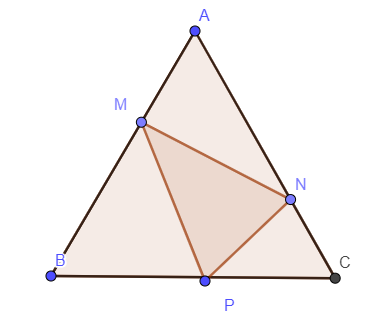
\includegraphics[width=0.3\linewidth]{anh1.png}
\end{figure}
\end{block}
\end{frame}


% 1.6 Phương pháp hình học
\begin{frame}{1.6 PHƯƠNG PHÁP HÌNH HỌC
\hspace{3cm}  70. Nguyễn Phương Thùy} 
%\framesubtitle{} 
\begin{block}{Giải:}
Dựng tam giác đều cạnh bằng một,$AM=x,PC=y,BN=z,$ như hình vẽ:\\Ta có :$S_{\Delta AMP} + S_{\Delta CPN} + S_{\Delta BMN} < S_{\Delta ABC} . $\\$ \Leftrightarrow \frac{1}{2}\sin{60^o}[x(1-y) + y(1-z) + z(1-x) ] < \frac{1}{2}\sin{60^o}.1.1.$\\ $\Leftrightarrow x(1-y) + y(1-z) + z(1-x) < 1.$(đpcm)

\begin{figure}
    \raggedleft
    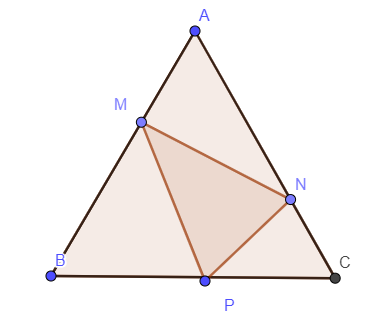
\includegraphics[width=0.25\linewidth]{anh1.png}
\end{figure}
\end{block}
\end{frame}

% 1.6 Phương pháp hình học
\begin{frame}{1.6 PHƯƠNG PHÁP HÌNH HỌC
\hspace{3cm}  70. Nguyễn Phương Thùy} 
%\framesubtitle{} 
\begin{block}{Bài toán 3:}
\textbf{Chứng minh bất đẳng thức Cauchy với hai số thực $a,b $ không âm.}\\
\end{block}
\end{frame}

% 1.6 Phương pháp hình học
\begin{frame}{1.6 PHƯƠNG PHÁP HÌNH HỌC
\hspace{3cm}  70. Nguyễn Phương Thùy} 
%\framesubtitle{} 
\begin{block}{Lời giải:}
\begin{figure}
    \centering
    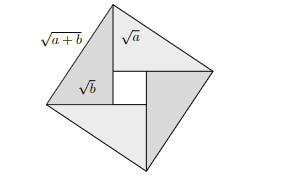
\includegraphics[width=0.7\linewidth]{anh2.png}
\end{figure}
\end{block}
\end{frame}


% 1.6 Phương pháp hình học
\begin{frame}{1.6 PHƯƠNG PHÁP HÌNH HỌC
\hspace{3cm}  70. Nguyễn Phương Thùy} 
%\framesubtitle{} 
\begin{block}{Lời giải:}\\Ta có : tổng diện tích của 4 tam giác vuông bên trong luôn bé hơn diện tích của hình vuông bao quanh có cạnh là $\sqrt{a+b}$,hay nói cách khác\\$(\sqrt{a+b})^2 \ge 4.\frac{1}{2}.\sqrt{a}.\sqrt{b} \Leftrightarrow a+b \ge \sqrt{ab} .$
\begin{figure}
    \raggedleft
    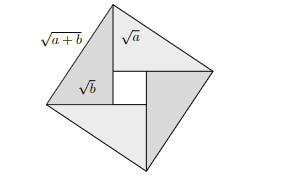
\includegraphics[width=0.5\linewidth]{anh2.png}
\end{figure}
\end{block}
\end{frame}





% \begin{frame}{1.7 PHƯƠNG PHÁP LƯỢNG GIÁC \hspace{3cm}  71. Bùi Anh Thư}  
%\framesubtitle{} 
\begin{block}{Một số dấu hiệu}
  +) Nếu $x^2+y^2=r^2, r>0$ thì ta đặt  $\left\{
    \begin{array}{cc}
        x=rcos\alpha\\
        y=rsin\alpha
    \end{array}
    \right.$
    với \alpha \in $[0;2\pi]$ \\
+) Nếu $\frac{x^2}{a^2}+\frac{y^2}{b^2}=r^2, a,b,r>0$ thì ta đặt $\left\{
    \begin{array}{cc}
        x=racos\alpha\\
        y=rbsin\alpha
    \end{array}
    \right.$
    với \alpha \in $[0;2\pi]$ \\
    +) Nếu $\frac{x^2}{a^2}+\frac{y^2}{b^2} \leq 1, a,b,>0$ thì ta đặt $\left\{
    \begin{array}{cc}
        x=racos\alpha\\
        y=rbsin\alpha
    \end{array}
    \right.$
    với $0\leq r\leq 1$ và \alpha \in $[0;2\pi]$ .\\
    \end{block} 
\end{frame}

\begin{frame}{1.7 PHƯƠNG PHÁP LƯỢNG GIÁC \hspace{3cm}  71. Bùi Anh Thư}  
%\framesubtitle{} 
\begin{block}{Một số dấu hiệu}
    +) Nếu $|x|\leq r$ thì đặt $x=rcos\alpha $ với \alpha \in $[0;\pi]$ hoặc $x=rsin\alpha$ với $\alpha \in [\frac{-\pi}{2};\frac{\pi}{2}]$\\
    \vspace{0,4cm}
    
    +) Nếu $|x|\geq r >0$ hoặc bài toán có chứa biểu thức $\sqrt{x^2+r^2}$ thì đặt $x=\frac{r}{cos\alpha}$ với $\alpha \in [0;\frac{\pi}{2}) \cup (\frac{\pi}{2};\pi]$ hoặc $x=\frac{r}{sin\alpha}$ với $\alpha \in (0;\pi)$\\
    \vspace{0,4cm}
    
    +) Nếu biến số $x$ không có điều kiện ràng buộc thì đặt $x=tan\alpha$ với $\alpha \in (-\frac{\pi}{2};\frac{\pi}{2})$.
\end{block} 
\end{frame}

\begin{frame}{1.7 PHƯƠNG PHÁP LƯỢNG GIÁC \hspace{3cm}  71. Bùi Anh Thư} 
%\framesubtitle{} 
\begin{block}{Bài toán 1}
Cho $x^2+y^2=2$. Chứng minh rằng $2(x^3-y^3)-3(x-y)\leq 2$\\
\end{block} \\
\pause
\vspace{0,2cm}

Giải:\\
Do $x^2+y^2=2$ nên ta có thể đặt $\left\{
    \begin{array}{cc}
        x=\sqrt{2}cos\alpha\\
        y=\sqrt{2}sin\alpha
    \end{array}
    \right.$ với $\alpha\in[0;2\pi]$\\
    \vspace{0,4cm}
    
    Khi đó $2(x^3-y^3)-3(x-y)=4\sqrt{2}(\cos^3{\alpha}-\sin^3{\alpha})-3\sqrt{2}(\cos{\alpha}-\sin{\alpha})$\\
    \vspace{0,4cm}
    $=\sqrt{2}[(4\cos^3{\alpha}-3\cos{\alpha})+(3\sin{\alpha}-4\sin^3{\alpha})]$\\
    \vspace{0,4cm}
    $=\sqrt{2}(\cos{3\alpha}+\sin{3\alpha})=2\sin{3\alpha+\frac{\pi}{4}}\leq 2$\\
    \vspace{0,4cm}
    
    Ta có điều phải chứng minh.
      \end{frame}
    

 \begin{frame}{1.7 PHƯƠNG PHÁP LƯỢNG GIÁC \hspace{3cm}  71. Bùi Anh Thư}  
%\framesubtitle{} 
\begin{block}{Đổi biến số đưa về bất đẳng thức tam giác}
   Nếu bài toán cho $x,y,x$ dương thỏa mãn $xy+yz+zx=1$ hoặc $x+y+z+2xyz=1$ hoặc biến đổi đưa về ràng buộc đó thì sử dụng các kết quả sau kết hợp với các BĐT cơ bản trong tam giác.\\
   \vspace{0,4cm}
   
   \textbf{Kết quả 1:} Với $x,y,z$ là các số thực dương thỏa mãn điều kiện $xy+yz+zx=1$ khi đó:\\
   \vspace{0,4cm}
   
   1.1. Tồn tại tam giác ABC sao cho\\
   $x=\tan \frac{A}{2}; y=\tan \frac{B}{2}; z= \tan \frac{C}{2}$.\\
   \vspace{0,4cm}
   
   1.2. Tồn tại tam giác nhọn ABC sao cho\\
   $x=\cot{A}; y=\cot{B}; z=\cot{C}$.\\
\end{block} 
\end{frame}
   
   \begin{frame}{1.7 PHƯƠNG PHÁP LƯỢNG GIÁC \hspace{3cm}  71. Bùi Anh Thư} 
%\framesubtitle{} 
\begin{block}{Đổi biến số đưa về bất đẳng thức tam giác}
   \textbf{Kết quả 2.} Với $x,y,z$ là các số thực dương thỏa mãn điều kiện $x+y+z=xyz$, khi đó:\\
   \vspace{0,4cm}
   
   2.1. Tồn tại tam giác nhọn ABC sao cho\\ $x=\tan A; y=\tan B; z= \tan C$.\\
   \vspace{0,4cm}
   
   2.2. Tồn tại tam giác ABC sao cho\\ $x=\cot{\frac{A}{2}}, y=\cot{\frac{B}{2}}; z=\cot{\frac{C}{2}}$\\
\end{block} 
\end{frame}

\begin{frame}{1.7 PHƯƠNG PHÁP LƯỢNG GIÁC \hspace{3cm}  71. Bùi Anh Thư} 
%\framesubtitle{} 
\begin{block}{Đổi biến số đưa về bất đẳng thức tam giác}
   \textbf{Kết quả 3.} Với $x,y,z$ là các số thực dương thỏa mãn điều kiện $x^2+y^2+z^2+2xyz=1$, khi đó:\\
   \vspace{0,4cm}
   
   3.1. Tồn tại tam giác nhọn ABC sao cho\\ $x=\cos{A}; y=\cos{B}; z= \cos{C}$.\\
   \vspace{0,4cm}
   
   3.2. Tồn tại tam giác ABC sao cho\\ $x=\sin{\frac{A}{2}}, y=\sin{\frac{B}{2}}; z=\sin{\frac{C}{2}}$\\
\end{block} 
\end{frame}


\begin{frame}{1.7 PHƯƠNG PHÁP LƯỢNG GIÁC \hspace{3cm}  71. Bùi Anh Thư} 
%\framesubtitle{} 
\begin{block}{Bài toán 2 (Poland 1999)}
   Cho $x,y,z>0$ thỏa mãn $x+y+z=1$. Chứng minh rằng $x^2+y^2+z^2+2\sqrt{3xyz}\leq 1$\\
   \end{block}
   \pause
   \vspace{0,2cm}
   
   Giải:\\
   Ta có: $x+y+z=1$\\
   $\leftrightarrow \sqrt{\frac{yz}{x}}.\sqrt{\frac{zx}{y}}+\sqrt{\frac{zx}{y}}.\sqrt{\frac{xy}{z}}+\sqrt{\frac{xy}{z}}.\sqrt{\frac{yz}{x}}=1$\\
   \vspace{0,4cm}
   
   Sử dụng kết quả 1.1, tồn tại tam giác ABC thỏa mãn:\\
    $\left\{
    \begin{array}{ccc}
        \sqrt{\frac{yz}{x}}=\tan\frac{A}{2}\\
        \sqrt{\frac{zx}{y}}=\tan\frac{B}{2}\\
        \sqrt{\frac{xy}{z}}=\tan\frac{C}{2}
        
    \end{array}
    \right.$ 
\end{frame}

\begin{frame}{1.7 PHƯƠNG PHÁP LƯỢNG GIÁC \hspace{3cm}  71. Bùi Anh Thư} 
%\framesubtitle{} 
Khi đó, BĐT cần chứng minh tương đương với\\
$\tan^2\frac{A}{2}.\tan^2\frac{B}{2}+\tan^2\frac{B}{2}.\tan^2\frac{C}{2}+\tan^2\frac{C}{2}.\tan^2\frac{A}{2}+2\sqrt{3}\tan\frac{A}{2}\tan\frac{B}{2}\tan\frac{C}{2}\leq 1$\\
\vspace{0,4cm}

$\leftrightarrow (\tan\frac{A}{2}\tan\frac{B}{2}+\tan\frac{B}{2}\tan\frac{C}{2}+\tan\frac{C}{2}\tan\frac{A}{2})^2+2\sqrt{3}\tan\frac{A}{2}\tan\frac{B}{2}\tan\frac{C}{2}\leq 1+2\tan\frac{A}{2}\tan\frac{B}{2}\tan\frac{C}{2}(\tan\frac{A}{2}+\tan\frac{B}{2}+\tan\frac{C}{2})$\\
\vspace{0,4cm}

$\leftrightarrow \tan\frac{A}{2}+\tan\frac{B}{2}+\tan\frac{C}{2}\geq \sqrt{3}$\\

\end{frame}

% % 1.8 Phương pháp quy nạp toán học
\begin{frame}{1.8 PHƯƠNG PHÁP QUY NẠP TOÁN HỌC \hspace{2cm}  72. Hà Anh Thư} 
%\framesubtitle{} 

\begin{block}{Nội dung phương pháp quy nạp toán học}
Có thể chứng minh một mệnh đề phụ thuộc vào số tự nhiên $n$ là đúng với mọi $n \ge n_0$ bằng phương pháp quy nạp toán học theo ba bước:
\pause
\begin{enumerate}
    \item Kiểm tra cụ thể mệnh để đúng với mọi $n = n_0$.
    \pause
    \item Giả sử mệnh đề đúng tới $n = k \in \mathbb{N}, k \ge n_0$.
    \pause
    \item Chứng minh mệnh đề đúng với $n = k + 1$ bằng cách sử dụng giả thiết và điều đã giả sử ở bước thứ hai (được gọi là giả thiết quy nạp). Khi đó kết luận mệnh đề đúng với mọi $n \ge n_0$.
\end{enumerate}
\end{block} 
\end{frame}
\begin{frame}{1.8 PHƯƠNG PHÁP QUY NẠP TOÁN HỌC \hspace{2cm}  72. Hà Anh Thư} 
\begin{block}{Ví dụ: Bài tập 1 trang 121}
Chứng minh rằng với $x > 0$ và số nguyên dương $n \ge 1$ ta có:
\begin{center}
    $e^x > 1 + \dfrac{x}{1!} + \dfrac{x^2}{2!} + ... + \dfrac{x^n}{n!}$
\end{center}
\pause
\begin{center}
    Giải:   
\end{center}
Xét $f_n(x) = e^x - 1 - \dfrac{x}{1!} - \dfrac{x^2}{2!} - ... - \dfrac{x^n}{n!}$.

Cần chứng minh $f_n(x) > 0 \forall x > 0, n \ge 1$.
\pause
\begin{enumerate}
    \item Với $n = 1, f_1(x) = e^x - 1- x \Rightarrow f_1'(x) = e^x - 1 > 0$ \\
    \pause
    Hàm số $f_1(x)$ đồng biến $\forall x > 0 \Rightarrow f_1(x) > f_1(0) = 0$. (đúng)
    \pause
    \item Giả sử đúng với $n = k$.
\end{enumerate}
\end{block}
\end{frame}
\begin{frame}{1.8 PHƯƠNG PHÁP QUY NẠP TOÁN HỌC \hspace{2cm}  72. Hà Anh Thư} 
\begin{block}{Ví dụ: Bài tập 1 trang 121}
\begin{enumerate}
    \setcounter{enumi}{2}
    \item Với $n = k + 1$. Cần chứng minh:
    \begin{center}
        $f_{k + 1}(x) = e^x - 1 - \dfrac{x}{1!} - \dfrac{x^2}{2!} - ... - \dfrac{x^k}{k!} - \frac{x^{k + 1}}{(k + 1)!} > 0$
    \end{center}
    \pause
    Thật vậy,
    $f_{k + 1}'(x) = e^x - 1 - \dfrac{x}{1!} - \dfrac{x^2}{2!} - ... - \dfrac{x^k}{k!} = f_k(x) > 0$ (Theo giả thiết quy nạp).
    \pause
    Hàm số $f_{k + 1}(x)$ đồng biến $\forall x > 0, n \ge 1 \Rightarrow f_{k + 1}(x) > f_{k + 1}(0) = 0$. (đúng) \\
    Vậy, ta có điều phải chứng minh.
\end{enumerate}
\end{block}

\end{frame}

\begin{frame}{1.8 PHƯƠNG PHÁP QUY NẠP TOÁN HỌC \hspace{2cm}  72. Hà Anh Thư} 
\begin{block}{Các bài toán phổ thông sử dụng phương pháp quy nạp toán học}
\textbf{Ví dụ 1:} Chứng minh bất đẳng thức $2^n > 2n + 1$ $(1)$ luôn đúng với mọi số tự nhiên $n \ge 3$ \\
\pause
\begin{center}
    Giải:
\end{center}
\begin{itemize}
    \item Khi $n = 3$ ta có $2^3 = 8 > 2.3 + 1 = 7$.
    \pause
    \item Giả sử $(1)$ đúng với $n = k \ge 3 (k \in \mathbb{N}) \Rightarrow 2^k > 2k + 1$ $(2)$. \\
        \pause
        $\Rightarrow$ Ta cần chứng minh $(2)$ đúng với $n = k + 1$. \\
        \pause
        $\Rightarrow 2^{k + 1} > 2(k + 1) + 1 \Leftrightarrow 2^{k + 1} > 2k + 3$ \\
        \pause
    \item Nhân cả 2 vế của $(2)$ với $2$ ta có: \\
        $2.2^k > 2k + 2k + 2 \Leftrightarrow 2^{k + 1} > 2k + 2k + 2$ $(3)$ \\
        \pause
        Vì $k \ge 3$ nên $2k \ge 6$. Do đó $(3) \Leftrightarrow 2^{k + 1} > 2k + 6 + 2 \Rightarrow 2^{k + 1} > 2k + 3$ \\
        $\Rightarrow$ Bất đẳng thức đúng với $n = k + 1$ $\Rightarrow$ Điều cần chứng minh.
\end{itemize}
\end{block}

\end{frame}

\begin{frame}{1.8 PHƯƠNG PHÁP QUY NẠP TOÁN HỌC \hspace{2cm}  72. Hà Anh Thư} 
\begin{block}{Các bài toán phổ thông sử dụng phương pháp quy nạp toán học}
\textbf{Ví dụ 2:} (Bất đẳng thức Bernoulli) Chứng minh bất đẳng thức $(1 + x)^n > 1 + nx$ $(1)$ luôn đúng với mọi số tự nhiên $x \ge -1, x \ne 0$ và với mọi số tự nhiên $n \ge 2$. \\
\pause
\begin{center}
    Giải:
\end{center}
\begin{itemize}
    \item Khi $n = 2$ ta có $(1 + x)^2 > 1 + 2x \Leftrightarrow x^2 > 0$ đúng do $x \ne 0$.
    \pause
    \item Giả sử $(1)$ đúng với $n = k \ge 2 (k \in \mathbb{N}) \Rightarrow (1 + x)^k > 1 + kx$ $(2)$. \\
        \pause
        $\Rightarrow$ Ta cần chứng minh $(2)$ đúng với $n = k + 1$. \\
        \pause
        Ta có $(1 + x)^{k + 1} = (1 + x)^k(1 + x) > (1 + kx)(1 + x)$ \\
        \pause
        Ta có $(1 + kx)(1 + x) =  1 + (k + 1)x + kx^2 > 1 + (k + 1)x$ \\
        $\Rightarrow$ Bất đẳng thức đúng với $n = k + 1$ $\Rightarrow$ Điều cần chứng minh.
\end{itemize}
\end{block}

\end{frame}

\begin{frame}{1.8 PHƯƠNG PHÁP QUY NẠP TOÁN HỌC \hspace{2cm}  72. Hà Anh Thư} 
\begin{block}{Các bài toán phổ thông sử dụng phương pháp quy nạp toán học}
\textbf{Ví dụ 3:} Chứng minh bất đẳng thức $(n!)^2 \ge n^n$ $(1)$ luôn đúng với mọi $n \in \mathbb{N}^*$. \\
\pause
\begin{center}
    Giải:
\end{center}
\begin{itemize}
    \item Trước hết ta chứng minh $n^n \ge (n + 1)^{n - 1}$ $(2)$ luôn đúng với mọi $n \in \mathbb{N}^*$ \\
    \pause
    \item Khi $n = 1$ ta có $1^1 \ge 2^0 \Leftrightarrow 1 \ge 1$ đúng. \\
    \pause
    \item Giả sử $(2)$ đúng với $n = k \in \mathbb{N}^* \Leftrightarrow k^k \ge (k + 1)^{k - 1} \Leftrightarrow \left(\dfrac{k}{k + 1}\right)^k \ge \dfrac{1}{k + 1}$ $(3)$ \\
        \pause
        $\Rightarrow$ Ta cần chứng minh $(3)$ đúng với $n = k + 1$. \\
        \pause
        Ta có $k^2 + 2k + 1 \ge k^2 + 2k \Rightarrow \dfrac{k + 1}{k + 2} \ge \dfrac{k}{k + 1} \Rightarrow \left(\dfrac{k + 1}{k + 2}\right)^k \ge \left(\dfrac{k}{k + 1}\right)^k \ge \dfrac{1}{k + 1}$ \\
        $\Rightarrow \left(\dfrac{k + 1}{k + 2}\right)^{k + 1} \ge \dfrac{1}{k + 1} \Rightarrow n^n \ge (n + 1)^{n - 1}$ đúng với $n \in \mathbb{N}^*$
\end{itemize}
\end{block}

\end{frame}

\begin{frame}{1.8 PHƯƠNG PHÁP QUY NẠP TOÁN HỌC \hspace{2cm}  72. Hà Anh Thư} 
\begin{block}{Các bài toán phổ thông sử dụng phương pháp quy nạp toán học}
\begin{itemize}
    \item Xét $(1)$ khi $n = 1$ ta có $(1!)^2 \ge 1^1 \Leftrightarrow 1 \ge 1$ đúng.
    \pause
    \item Giả sử $(1)$ đúng với $n = k \in \mathbb{N}^* \Leftrightarrow (k!)^2 \ge k^k$ $(4)$ \\
        \pause
        $\Rightarrow$ Ta cần chứng minh $(4)$ đúng với $n = k + 1$ $\Leftrightarrow \left[(k + 1)!\right]^2 \ge (k + 1)^{k + 1}$ \\
        \pause
        Ta có $\left[(k + 1)!\right]^2 = \left[k!(k + 1)\right]^2 = (k!)^2(k + 1)^2 \ge k^k(k + 1)^2$ \\
        \pause
        Áp dụng $(2)$ ta có $k^k(k + 1)^2 > (k + 1)^{k - 1}(k + 1)^2 = (k + 1)^{k + 1}$ \\
        $\Leftrightarrow$ Bất đẳng thức đúng với $n = k + 1$ $\Rightarrow$ Điều cần chứng minh.
\end{itemize}
\end{block}

\end{frame}

\begin{frame}{1.8 PHƯƠNG PHÁP QUY NẠP TOÁN HỌC \hspace{2cm}  72. Hà Anh Thư} 
\begin{block}{Các bài toán phổ thông sử dụng phương pháp quy nạp toán học}
\textbf{Ví dụ 4:} (Vô địch Toán Matxcova 1984) Cho $x_1, x_2, ..., x_n$ là $n$ số không âm $(n \in \mathbf{Z}, n \ge 4)$, tổng của chúng bằng $1$. Chứng minh rằng $x_1x_2 + x_2x_3 + ... + x_nx_1 \le \dfrac{1}{4}$ $(1)$ \\
\pause
\begin{center}
    Giải:
\end{center}
\begin{itemize}
    \item $(1) \Leftrightarrow (x_1 + x_2 + ... + x_n)^2 \ge 4(x_1x_2 + x_2x_3 + ... + x_nx_1)$
    \pause
    \item Khi $n = 4$ ta có $(x_1 + x_2 + x_3 + x_4)^2 \ge 4$. $\Leftrightarrow (x_1 - x_2 + x_3 - x_4)^2 \ge 0$ đúng với $n = 4$.
    \pause
    \item Giả sử $(1)$ đúng với $n = k \ge 4 (k \in \mathbb{N})$ \\
        $\Rightarrow (x_1 + x_2 + ... + x_k)^2 \ge 4(x_1x_2 + x_2x_3 + ... + x_kx_1)$ $(2)$ \\
        \pause
        $\Rightarrow$ Ta cần chứng minh $(2)$ đúng với $n = k + 1$. \\
        $(x_1 + x_2 + ... + x_k + x_{k + 1})^2 \ge 4(x_1x_2 + x_2x_3 + ... + x_kx_{k + 1} + x_{k + 1}x_1)$
\end{itemize}
\end{block}

\end{frame}

\begin{frame}{1.8 PHƯƠNG PHÁP QUY NẠP TOÁN HỌC \hspace{2cm}  72. Hà Anh Thư} 
\begin{block}{Các bài toán phổ thông sử dụng phương pháp quy nạp toán học}
\begin{itemize}
    \item Vì tổng hai vế của bất đẳng thức này là vòng tròn theo chỉ số, nên ta có thể giả thiết $x_{k + 1} \le x_i, i = \overline{\rm 1, k}$.
    \pause
    \item Ta có $(x_1 + x_2 + ... + x_k + x_{k + 1})^2 = (x_1 + x_2 + ... + (x_k + x_{k + 1}))^2$ \\
        $\ge 4[x_1x_2 + x_2x_3 + ... + x_{k - 1}(x_k + x_{k + 1}) + (x_k + x_{k + 1})x_1]$
    \pause
    \item Mà $[x_1x_2 + x_2x_3 + ... + x_{k - 1}(x_k + x_{k + 1}) + (x_k + x_{k + 1})x_1]$ \\
        $= (x_1x_2 + x_2x_3 + ... + x_kx_{k + 1} + x_{k + 1}x_1) + x_{k - 1}x_{k+1} + x_k(x_1 - x_{k + 1})$ \\
    \pause
    \item Vì $x_i \ge 0$ và $x_1 - x_{k + 1} \ge 0$, nên ta có \\
        $[x_1x_2 + x_2x_3 + ... + x_{k - 1}(x_k + x_{k + 1}) + (x_k + x_{k + 1})x_1]$ \\
        $\ge (x_1x_2 + x_2x_3 + ... + x_kx_{k + 1} + x_{k + 1}x_1)$.
    \pause
    \item Vậy $(x_1 + x_2 + ... + x_k + x_{k + 1})^2 \ge 4(x_1x_2 + x_2x_3 + ... + x_kx_{k + 1} + x_{k + 1}x_1)$
        $\Rightarrow$ Bất đẳng thức đúng với $n = k + 1$ $\Rightarrow$ Điều cần chứng minh.
\end{itemize}
\end{block}
\end{frame}

% % 1.9. Sử dụng hàm đơn điệu
\begin{frame}{1.9 SỬ DỤNG HÀM ĐƠN ĐIỆU\hspace{2cm}  73. Nguyễn Thị Hà Thương} 
%\framesubtitle{} 
\begin{block}{\textbf{Định lí}}
Cho hàm số $y=f(x)$ xác định, liên tục trong khoảng $(a;b)$. Khi đó:\\
\begin{itemize}
    \item Nếu $f'(x)>0 \quad \forall x \in (a;b)$ thì $f(x)$ đồng biến trên khoảng $(a;b)$.
    \item Nếu $f'(x)<0 \quad \forall x \in (a;b)$ thì $f(x)$ nghịch biến trên khoảng $(a;b)$.
\end{itemize}
    
\end{block} 
\pause
\textbf{Nhận xét.}\\
Việc chứng minh $A \geq B$ được đưa về xét hàm $A-B$ qua đạo hàm.\\
$\rightarrow$ \text{Từ tính đồng biến hay nghịch biến của $A-B$ ta suy ra bất đẳng thức.}
\end{frame} 

\begin{frame}{1.9 SỬ DỤNG HÀM ĐƠN ĐIỆU\hspace{2cm}  73. Nguyễn Thị Hà Thương} 
%\framesubtitle{} 
\begin{block}{Ví dụ}
Chứng minh: $sinx<x<tanx, \forall x\in (0;\frac{\pi}{2})$
\end{block}
\pause

Xét hàm số $f(x)=sinx-x$ trên khoảng $(0;\frac{\pi}{2})$\\
$f'(x)=cosx-1 < 0$ $\Rightarrow$ {$f(x)$ \quad \text{nghịch biến}}\\
$0<x<\frac{\pi}{2}$ $\Rightarrow$ {$f(0) > f(x)$} \quad $\Rightarrow${$0 > sinx - x$}\quad hay \quad $x > sinx$ \quad $(1)$\\
\pause
Xét hàm số $g(x)=tanx-x$ trên khoảng $(0;\frac{\pi}{2})$\\
$g'(x)=\frac{1}{cos^2x}-1=\frac{1-cos^2x}{cos^2x} > 0$ $\Rightarrow${$g(x)$ \quad \text{đồng biến}}\\
$0<x<\frac{\pi}{2}$ $\Rightarrow${$g(0) < g(x)$} \quad $\Rightarrow${$0 < tanx - x$}\quad hay \quad $x < tanx$ \quad $(2)$\\

\indent Từ $(1)$ và $(2)$ $\Rightarrow${\text{đpcm}}
\end{frame} 

\begin{frame}{1.9 SỬ DỤNG HÀM ĐƠN ĐIỆU\hspace{2cm}  73. Nguyễn Thị Hà Thương} 
%\framesubtitle{} 
\begin{block}{\textbf{Bài tập đề xuất}}
\large Cho $n\in\mathbb{N}^*$, chứng minh:\\
\centering \large $\frac{1}{\sqrt{1^2+1}}+\frac{1}{\sqrt{2^2+2}}+...+\frac{1}{\sqrt{n^2+n}}>\ln{(n+1)}$
\end{block}

\pause
\large Xét hàm số $f(x)=\frac{1}{\sqrt{x^2+x}}-\ln{(x+1)}+\ln{x}, \forall x \geq 1$
\end{frame} 

\begin{frame}{1.9 SỬ DỤNG HÀM ĐƠN ĐIỆU\hspace{2cm}  73. Nguyễn Thị Hà Thương} 
%\framesubtitle{}
\large $f(x)=\frac{1}{\sqrt{x^2+x}}-\ln{(x+1)}+\ln{x}, \forall x \geq 1$\\
\large $f'(x)= \frac{\frac{-2x-1}{2\sqrt{x^2+x}}}{x^2+x} - \frac{1}{x+1} + \frac{1}{x} = \frac{2\sqrt{x^2+x}-2x-1}{2(x^2+x)\sqrt{x^2+x}} < 0, \forall x \geq 1 $
\pause
\begin{center}
    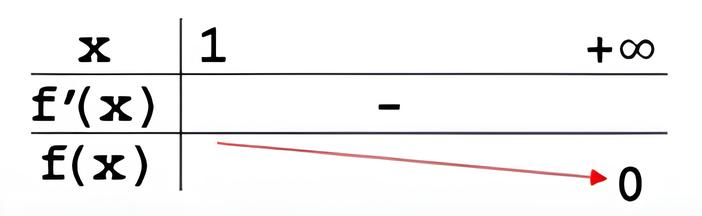
\includegraphics[scale=0.2]{bbt (1.9).JPG}
\end{center}
\pause
\large Suy ra $f(x)>0,\forall x \geq 1 $\\
\large nên $\frac{1}{\sqrt{x^2+x}} > \ln{(x+1)} - \ln{x}$
\end{frame}

\begin{frame}{1.9 SỬ DỤNG HÀM ĐƠN ĐIỆU\hspace{2cm}  73. Nguyễn Thị Hà Thương} 
	%\framesubtitle{}
		Do $\frac{1}{\sqrt{x^2+x}} > \ln{(x+1)} - \ln{x}$, ta có:\\
		$\frac{1}{\sqrt{1^2+1}} > \ln{2} - \ln{1}$\\
		$\frac{1}{\sqrt{2^2+2}} > \ln{3} - \ln{2}$\\
		...\\
		$\frac{1}{\sqrt{n^2+n}} > \ln{(n+1)} - \ln{n}$\\
$\Rightarrow$ $\frac{1}{\sqrt{1^2+1}}+\frac{1}{\sqrt{2^2+2}}+...+\frac{1}{\sqrt{n^2+n}} > \ln{(n+1)} - \ln{1} = \ln{(n+1)}$ $\Rightarrow$ {\text{đpcm.}}
\end{frame}

\begin{frame}{1.9 SỬ DỤNG HÀM ĐƠN ĐIỆU\hspace{2cm}  73. Nguyễn Thị Hà Thương}
\begin{block}{\textbf{Bài tập tham khảo} (Thi HSG Quốc gia 1992)}
Chứng minh rằng, với mọi số tự nhiên $n>1$ ta có:\\
\centering $\sqrt[n]{1+\frac{\sqrt[n]{n}}{n}}+\sqrt[n]{1-\frac{\sqrt[n]{n}}{n}} < 2$
\end{block}
\pause
Đặt $x=\frac{\sqrt[n]{n}}{n} \in (0;1)$. Bất đẳng thức cần chứng minh trở thành:\\
\begin{center}
$\sqrt[n]{1+x}+\sqrt[n]{1-x} < 2, \forall x\in (0;1)$.
\end{center}
\pause
Xét hàm số $f(x)=\sqrt[n]{1+x}+\sqrt[n]{1-x}$ liên tục trên khoảng $(0;1)$ có:\\
$f'(x)= \frac{1}{n}(\frac{1}{\sqrt[n]{(1+x)^{n-1}}}-\frac{1}{\sqrt[n]{(1-x)^{n-1}}})<0, \forall x \in (0;1)$\\
Vậy $f(x)$ nghịch biến trên $(0;1)$ nên $f(x)<f(0)=2 \Rightarrow \text{đpcm}$
\end{frame}


% % 1.10 Sử dụng định lý Rolle
\begin{frame}{1.10 SỬ DỤNG ĐỊNH LÝ ROLLE \hspace{4cm}  74. Hồ Hoàng Trang} 
%\framesubtitle{} 
	
		\begin{block}{Nhắc lại định lý Rolle}
			Cho $f$ là hàm xác định và liên tục trên đoan $\left[a;b\right]$ và có đạo hàm tại mọi điểm $x \in \left(a;b\right)$. Nếu $f(a)=f(b)$ thì tồn tại ít nhất một điểm $c\in \left(a;b\right)$ để $f'(c)=0$.
		\end{block}
\end{frame}
\begin{frame}{1.10 SỬ DỤNG ĐỊNH LÝ ROLLE \hspace{4cm}  74. Hồ Hoàng Trang}
		
			\begin{block}{Ý nghĩa của định lý Rolle}
				Cho hàm $f$ liên tục tại đoạn $\left[a;b\right]$ có đạo hàm trên $\left(a;b\right)$ và $f(a)=f(b)$, hai điểm $A(a;f(a))$ và $B(b;f(b))$. Lúc đó trên cung AB của đồ thị có ít nhất một điểm C mà tiếp tuyến tại đó của đồ thị cùng phương với trục hoành.
			\end{block}
\pause
\begin{center}
    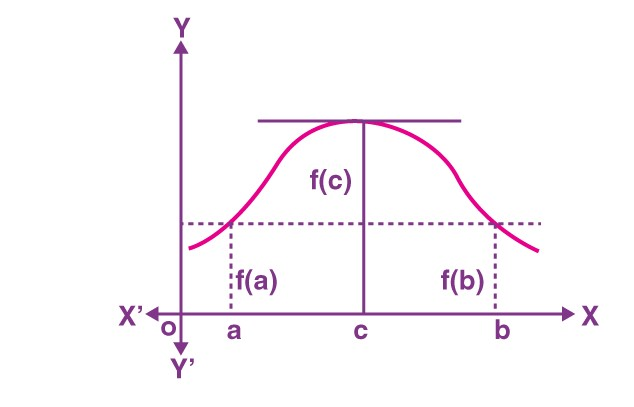
\includegraphics[scale=0.5]{rolle.jpg}
\end{center}
		\end{frame}
 \begin{frame}{1.10 SỬ DỤNG ĐỊNH LÝ ROLLE \hspace{4cm}  74. Hồ Hoàng Trang}
  \begin{minipage}{0.5\linewidth}
 \begin{block}{Ví dụ 1:}
     Cho hàm số $f(x)=x^2-5x+3$ trên đoạn $\left[0;5\right]$.\\
     \pause
     + Ta thấy hàm $f(x)$ xác định và liên tục trên $\left[0;5\right]$.\\
     \pause
     + Ta có $f(0)=0^2-5.0+3=3$, $f(5)=5^2-5.5+3=3$.\\ Khi đó ta có $f(0)=f(5)=3$\\
     \pause
     + Ta có $f'(x)=2x-5=0\Leftrightarrow x=\dfrac{5}{2}$.\\
     Mà ta có $\dfrac{5}{2} \in (0; 5)$.\\
     \pause
     Vậy hàm số thỏa mãn định lý Rolle.
 \end{block}
 
 \end{minipage}\qquad
 \begin{minipage}{0.4\linewidth}
			\includegraphics[scale=1]{đothibacba.png}
\end{minipage}
\end{frame}
\begin{frame}{{1.10 SỬ DỤNG ĐỊNH LÝ ROLLE \hspace{4cm}  74. Hồ Hoàng Trang}}

    \begin{minipage}{0.5\linewidth}
    \begin{block}{Ví dụ 2:}
    Cho hàm số $f(x)=sinx$ trên đoạn $\left[0;2\pi\right].$\\
    \pause
    + Ta thấy hàm $f(x)$ xác định và liên tục trên $\left[0;2\pi\right]$.\\
    \pause
    + Ta có $f(0)=sin(0)=0$, $f(2\pi)=sin(2\pi)=0$.\\ Khi đó ta có $f(0)=f(2\pi)=0$\\
    \pause
    + Ta có $f'(x)=cosx=0\Leftrightarrow x=\dfrac{\pi}{2}+k\pi$ với $k\in \mathbb{Z}$.\\
     Mà ta có $\dfrac{\pi}{2}, \dfrac{3\pi}{2} \in (0; 2\pi)$ là 2 nghiệm của hàm $f'(x)$.\\
     \pause
     Vậy hàm số thỏa mãn định lý Rolle.
    \end{block}
    \end{minipage}\qquad
\begin{minipage}{0.4\linewidth}
			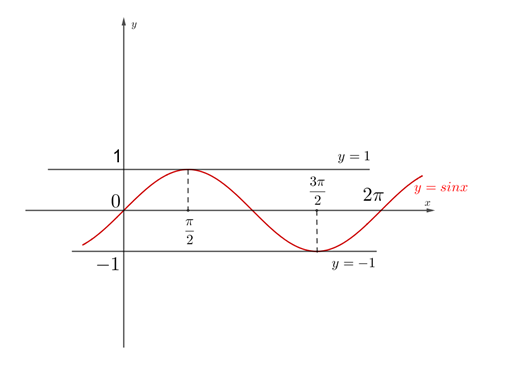
\includegraphics[scale=0.57]{y=sinx.png}
\end{minipage}

    \end{frame}

\begin{frame}

 \begin{block}{Hệ quả định lý Rolle}
 Nếu đa thức $f(x)$ liên tục và có $n$ $(n\ge 1)$ nghiệm phân biệt thuộc khoảng $(a,b)$ thì đạo hàm của nó $f'(x)$ là đa thức có ít nhất $n-1$ nghiệm thuộc khoảng $(a,b)$. Các đa thức $f^{(k)}(x)$ $(1 \le k\le n)$ có ít nhất $n-k$ nghiệm phân biệt thuộc khoảng $(a,b)$.
 \end{block}
 \pause
 \textbf{Giải thích hệ quả:} $f(x)$ có $n$ nghiệm phân biệt $x_1,x_2,\cdots ,x_n$ hay $f(x_1)=f(x_2)=\cdots=f(x_n)=0$ $(x_1,x_2,\cdots, x_n \in (a,b))$.\\
 \pause
 Ta có $f(x)$ liên tục trên $(a,b)$ nên áp dụng định lý Rolle cho hàm $f(x)$ trên các đoạn $[x_1,x_2];[x_2, x_3],\cdots[x_{n-1}, x_n]$ ta có tồn tại các điểm:\\
 \pause 
 $y_1\in \left[x_1,x_2\right]$\\
  $y_2\in \left[x_2,x_3\right]$\\
  $\cdots$\\
   $y_{n-1}\in \left[x_{n-1},x_n\right]$\\
   là nghiệm của hàm $f'(x)$. Vậy f'(x) có ít nhất $n-1$ nghiệm thuộc $(a,b)$.\\
   \pause 
   Tiếp tục áp dụng định lý Rolle với hàm $f'(x)$ , rồi $f''(x)$ ta chứng minh được đa thức $f^{(k)}(x)$ $(1 \le k\le n)$ có ít nhất $n-k$ nghiệm phân biệt thuộc khoảng $(a,b)$
\end{frame}

\begin{frame}{{1.10 SỬ DỤNG ĐỊNH LÝ ROLLE \hspace{4cm}  74. Hồ Hoàng Trang}}
    \textbf{Bài toán 1 (Đề olympic Nga):} Cho phương trình:\\
    $$a_0x^n+a_1x^{n-1}+\cdots+a_{n-1}x+a_n=0.(a_i\ne 0, i=1,2,\cdots n)$$
    có n nghiệm phân biệt. Chứng minh rằng:
    $$(n-1)a_1^2>2na_0a_2$$.
    \pause
    \begin{block}{Chứng minh}
    \pause
        Xét đa thức $f(x)=a_0x^n+a_1x^{n-1}+\cdots+a_{n-1}x+a_n$.\\
        \pause
        Ta có $f(x)$ khả vi trên $\mathbb{R}$.\\ Vì $f(x)$ có $n$ nghiệm phân biệt, nên theo hệ quả định lý Rolle, ta có:\\
        $f'(x)$ có ít nhất $n-1$ nghiệm,\\
        \pause
        $f''(x)$ có ít nhất $n-2$ nghiệm,\\
        $\cdots$\\
        \pause
        $f^{(n-2)}(x)$ có ít nhất $2$ nghiệm,\\
        

         \end{block}
\end{frame}
\begin{frame}
\begin{block}

    Mặt khác, ta có $f^{(n-2)}(x)=\dfrac{n!}{2}a_0x^2+(n-1)!a_1x+(n-2)!a_2$\\
     $\Rightarrow$ $f^{(n-2)}$ có 2 nghiệm phân biệt:\\
     \pause
        $\Leftrightarrow$ $\Delta'>0$\\
        $\Leftrightarrow$ $\left[(n-1)!a_1\right]^2-2n!a_0(n-2)!a_2>0$\\
        $\Leftrightarrow$ $(n-1)a_1^2>2na_0a_2.$ (đpcm)
\end{block}
\end{frame}
\begin{frame}{{1.10 SỬ DỤNG ĐỊNH LÝ ROLLE \hspace{4cm}  74. Hồ Hoàng Trang}}
	\textbf{Bài toán 2:}
	Cho $a,b,c,d>0$. Chứng minh rằng: \\$\sqrt[3]{\dfrac{abc+abd+acd+bcd}{4}}\le \sqrt{\dfrac{ab+ac+ad+bc+bd+cd}{6}}$\\
	\pause
	\begin{block}{Chứng minh}
    \textbf{Nhận xét:} Ta thấy $abc+abd+acd+bcd$ và $ab+ac+ad+bc+bd+cd$ là các đa thức đối xứng cơ bản của $a,b,c,d$.\\
    \pause
        Giả sử $0< a\le b \le c  \le d$.\\
		Xét hàm số $F(x)=(x-a)(x-b)(x-c)(x-d)$\\
  \pause
		Khi đó $F(a)=F(b)=F(c)=F(d)=0$\\
  \pause
		Ta có $F(x)$ là hàm khả vi trên $\mathbb{R}$\\
  \pause
  Nên áp dụng định lý Rolle cho hàm $F(x)$ ta được:\\ $F'(x)$ có 3 nghiệm $y_1,y_2,y_3$ lần lượt thuộc các đoạn $\left[a,b\right]$, $\left[b,c\right]$, $\left[c,d\right]$ hay $a\le y_1 \le b \le y_2 \le c \le y_3 \le d$.\\
  \pause
   
	\end{block}
\end{frame} 
\begin{frame}
\begin{block}{}
Ta có $F(x)= x^4-(a+b+c+d)x^3+(ab+ac+ad+bc+bd+cd)x^2-(abc+abd+acd+bcd)x+abcd$\\
\pause
  Ta đặt:\\
   $T_1=a+b+c+d, T_2=ab+ac+ad+bc+bd+cd, T_3=abc+abd+acd+bcd, T_4=abcd$\\
Khi đó $F(x)=x^4-T_1x^3+T_2x^2-T_3x+T_4$\\
   \pause
    $\Longrightarrow F'(x)=4x^3-3T_1x^2+2T_2x-T_3$\\
    \pause
    Hàm $F'(x)$ có 3 nghiệm dương $y_1, y_2, y_3$. Theo định lý Viet ta có:\\
    $y_1y_2+y_2y_3+y_3y_1=\dfrac{T_2}{2}$; $y_1y_2y_3=\dfrac{T_3}{4}$.\\
    \pause
    Áp dụng BĐT Côsi ta có:\\
    $\dfrac{1}{3}(y_1y_2+y_2y_3+y_3y_1)\ge \sqrt[3]{(y_1y_2y_3)^2}$\\
    \pause
    $\Longrightarrow \dfrac{T_2}{6}\ge \sqrt[3]{\left(\dfrac{T_3}{4}\right)^2} $
     $\Longrightarrow  \sqrt[3]{\left(\dfrac{T_3}{4}\right)} \le \sqrt{\dfrac{T_2}{6}} $\\
     hay $\sqrt[3]{\dfrac{abc+abd+acd+bcd}{4}}\le \sqrt{\dfrac{ab+ac+ad+bc+bd+cd}{6}}$ (đpcm).
\end{block}
\end{frame}

\begin{frame}{{1.10 SỬ DỤNG ĐỊNH LÝ ROLLE \hspace{4cm}  74. Hồ Hoàng Trang}}
  \textbf{Bài toán 3:} (Đề thi quốc gia 1996) Cho $a,b,c,d \ge 0$ thỏa mãn:  $2(ab+ac+ad+bc+bd+cd)+abc+abd+acd+bcd=16$\\
  Chứng minh rằng: $a+b+c+d \ge \dfrac{2}{3}(ab+ac+ad+bc+bd+cd)$
  \pause
  \begin{block}{Chứng minh}
  \pause
    Tương tự bài toán 1 ta xét hàm $F(x)=(x-a)(x-b)(x-c)(x-d)=x^4-T_1x^3+T_2x^2-T_3x+T_4$.\\
    Trong đó:\\
   $T_1=a+b+c+d, T_2=ab+ac+ad+bc+bd+cd, T_3=abc+abd+acd+bcd, T_4=abcd$\\
   \pause
   Ta có $F'(x)=4x^3-3T_1x^2+2T_2x-T_3$.\\
   \pause
    Áp dụng định lý Rolle ta được:\\ 
    $F'(x)$ có 3 nghiệm $x_1, x_2, x_3$ trên các đoạn $\left[a,b\right]$, $\left[b,c\right]$, $\left[c,d\right]$ và $a\le x_1 \le b \le x_2 \le c \le x_3 \le d$.\\
    \end{block}
\end{frame}
    \begin{frame}
    \begin{block}
        
        Theo định lý Viet ta có:\\
    $x_1+x_2+x_3=\dfrac{3T_1}{4} $, 
    $x_1x_2+x_2x_3+x_3x_1=\dfrac{T_2}{2}$, $x_1x_2x_3=\dfrac{T_3}{4}$\\
    \pause
    Từ giả thiết ta có $2T_2+T_3=16$ \\
    $\Leftrightarrow 4(x_1x_2+x_2x_3+x_1x_3)+4x_1x_2x_3=16$\\
     $\Leftrightarrow x_1x_2+x_2x_3+x_1x_3+x_1x_2x_3=4$ (1)\\
     \pause
     Ta sẽ chứng minh bất đẳng thức trên bằng phương pháp biến đổi tương đương.\\
     \pause
     Từ giả thiết ta có 
      $a+b+c+d \ge \dfrac{2}{3}(ab+ac+ad+bc+bd+cd)$\\
      hay $T_1 \ge \dfrac{2}{3}T_2\Leftrightarrow \dfrac{4}{3}(x_1+x_2+x_3)\le \dfrac{2}{3}.2(x_1x_2+x_2x_3+x_3x_1)$\\
      $\Leftrightarrow x_1+x_2+x_3\ge x_1x_2+x_2x_3+x_3x_1$(*)\\
      \pause
       Ta có $x_1, x_2, x_3$ là các số không âm, nên từ (1) suy ra tồn tại ít nhất 2 số lớn hơn 0, giả sử $x_1, x_2>0$.\\
       Khi đó từ (1) ta rút $x_3=\dfrac{4-x_1x_2}{x_2+x_1+x_1x_2}$.\\
       
    \end{block}
    \end{frame}
\begin{frame}{1.10 SỬ DỤNG ĐỊNH LÝ ROLLE \hspace{4cm}  74. Hồ Hoàng Trang}
\begin{block}

    Khi đó $(*)\Leftrightarrow x_1+x_2+\dfrac{4-x_1x_2}{x_2+x_1+x_1x_2} \ge 4-x_1x_2\dfrac{4-x_1x_2}{x_1+x_2+x_1x_2}$
     $\Leftrightarrow (x_1+x_2)^2+x_1x_2(x_1+x_2)+4-x_1x_2\ge 4(x_1+x_2)+4x_1x_2-4x_1x_2+x_1^2x_2^2$\\
     $\Leftrightarrow (x_1+x_2-2)^2 \ge x_1x_2(1-x_1)(1-x_2)$ (**).\\
     \pause
     Nếu $(1-x_1)(1-x_2) \le 0$ thì (**) đúng.\\
     \pause
     Nếu $(1-x_1)(1-x_2) > 0$ thì ta có: $0<(1-x_1)(1-x_2)\le \dfrac{1}{4}(2-x_1-x_2)^2$ (1)\\
     Và ta có $x_3=\dfrac{4-x_1x_2}{x_1+x_2+x_1x_2} \Rightarrow 0<x_1x_2\le 4$ (2)\\
     Từ (1) và (2), suy ra (**) đúng.\\
     \pause
     Vậy (*) đúng hay $x_1+x_2+x_3\le x_1x_2+x_2x_3+x_3x_1$\\
     Hay $T_1 \le \dfrac{2}{3} T_2$ hay $a+b+c+d\le \dfrac{2}{3}(ab+ac+ad+bc+bd+cd)$(đpcm).
     
\end{block}
       
\end{frame}
\begin{frame}{1.10 SỬ DỤNG ĐỊNH LÝ ROLLE \hspace{4cm}  74. Hồ Hoàng Trang}
    \begin{block}{Bài toán tổng quát từ bài toán 2:}
Cho $x_i>0$ và $T_k=\displaystyle \sum_{1\le i_1 < i_2< \cdots <i_k\le n}x_{i_1}x_{i_2}\cdots x_{i_k}$. Chứng minh rằng:
\begin{center}
	$\dfrac{T_1}{C^1_{n}}\ge \sqrt{\dfrac{T_2}{C^2_{n}}}\ge \sqrt[3]{\dfrac{T_3}{C^3_{n}}}\ge \cdots\ge \sqrt[n]{\dfrac{T_n}{C^n_{n}}}$.
\end{center}
\end{block}
\end{frame}

  
 

% % 2.1 Hàm lồi
\begin{frame}{2.1 HÀM LỒI. \hspace{6cm}  75. Nguyễn Thị Thu Trang.} 
%\framesubtitle{} 
\begin{block}{Khái niệm hàm lồi: }
Hàm $y=f(x)$ được gọi là \textit{hàm lồi (lồi xuống dưới)} trong khoảng $(a; b)$ nếu với mọi $x_1, x_2 \in (a; b)$ và mọi số thực $\alpha_1 , \alpha_2 \ge 0, \alpha_1 +\alpha_2 = 1 $, ta có:
\begin{center}
    $\alpha_1 f(x_1) +\alpha_2 f(x_2) \ge f(\alpha_1 x_1 + \alpha_2 x_2).$
\end{center}
Hàm $y=f(x)$ được gọi là \textit{hàm lõm} trong khoảng $(a; b)$ nếu $y=-f(x)$ là hàm lồi.
\end{block} 
\end{frame} 
\begin{frame}{2.1 HÀM LỒI. \hspace{6cm}  75. Nguyễn Thị Thu Trang.} 
%\framesubtitle{} 
\begin{block}{Ví dụ 1: }
Hàm $f: \mathbb{R} \longrightarrow \mathbb{R}$\\
\hspace{1cm} $x\longmapsto f(x)= x^2$ là hàm lồi.
\end{block} 
\begin{center}
    \includegraphics[scale=0.25]{Screenshot (373).png}
\end{center}
\end{frame}
\begin{frame}{2.1 HÀM LỒI. \hspace{6cm}  75. Nguyễn Thị Thu Trang.} 
%\framesubtitle{} 
\begin{block}{Ví dụ 1: }
Hàm $f: \mathbb{R} \longrightarrow \mathbb{R}$\\
\hspace{1cm} $x\longmapsto f(x)= x^2$ là hàm lồi.
\end{block} 
Xét $x,y \in \mathbb{R}; \alpha \in [0; 1]$ ta có: \\$f(\alpha x + (1- \alpha)y) - \alpha f(x) - (1-\alpha) f(y)$\\
\vspace{2cm}
$f(\alpha x + (1- \alpha)y)\leq \alpha f(x) + (1-\alpha) f(y)$ với mọi $x, y \in \mathbb{R}, \alpha \in [0; 1]$\\
$\Rightarrow$  Hàm $f$ lồi.
\end{frame}
\begin{frame}{2.1 HÀM LỒI .\hspace{6cm}  75. Nguyễn Thị Thu Trang.} 
%\framesubtitle{} 
\begin{block}{Ví dụ 1: }
Hàm $f: \mathbb{R} \longrightarrow \mathbb{R}$\\
\hspace{1cm} $x\longmapsto f(x)= x^2$ là hàm lồi.
\end{block} 
Xét $x,y \in \mathbb{R}; \alpha \in [0; 1]$ ta có: \\$f(\alpha x + (1- \alpha)y) - \alpha f(x) - (1-\alpha) f(y)$\\
\pause
$= [\alpha x + (1- \alpha) y ]^2 - \alpha x^2 - (1-\alpha) y^2$ \\
\pause
$= (\alpha^2 -\alpha) x^2 + 2\alpha (1-\alpha) xy + (\alpha^2-\alpha) y^2$\\
\pause
$= \alpha(\alpha-1)(x^2- 2xy+y^2)$\\
\pause
$=\alpha(\alpha-1)(x-y)^2 \leq 0$\\
$\Rightarrow f(\alpha x + (1- \alpha)y)\leq \alpha f(x) + (1-\alpha) f(y)$ với mọi $x, y \in \mathbb{R}, \alpha \in [0; 1]$\\
$\Rightarrow$  Hàm $f$ lồi.
\end{frame}
\begin{frame}{2.1 HÀM LỒI. \hspace{6cm}  75. Nguyễn Thị Thu Trang.}
\begin{block}{Ví dụ 2: }
Hàm $h: \mathbb{R} \longrightarrow \mathbb{R}$\\
\hspace{1.2cm} $x\longmapsto h(x)= x^3$ \textbf{không} là hàm lồi.
\end{block}
\begin{center}
    \includegraphics[scale=0.5]{1561336492492_5.png}
\end{center}
\end{frame}
\begin{frame}{2.1 HÀM LỒI. \hspace{6cm}  75. Nguyễn Thị Thu Trang.}
\begin{block}{Ví dụ 2: }
Hàm $h: \mathbb{R} \longrightarrow \mathbb{R}$\\
\hspace{1.2cm} $x\longmapsto h(x)= x^3$ \textbf{không} là hàm lồi.
\end{block}
\textbf{Mục tiêu:} Chỉ ra \textbf{tồn tại} $x,y \in \mathbb{R}, \alpha \in [0,1]$ thỏa mãn: $h(\alpha x+(1 -\alpha)y) > \alpha h(x) + (1-\alpha)h(y)$\\
\end{frame}
\begin{frame}{2.1 HÀM LỒI. \hspace{6cm}  75. Nguyễn Thị Thu Trang.}
\begin{block}{Ví dụ 2: }
Hàm $h: \mathbb{R} \longrightarrow \mathbb{R}$\\
\hspace{1.2cm} $x\longmapsto h(x)= x^3$ \textbf{không} là hàm lồi.
\end{block}
Với $x = -3, y = 1, \alpha = \dfrac{1}{2}$ ta có:\\
$h(\alpha x+(1 -\alpha)y) = h(-1)=-1 $\\
$\alpha h(x) + (1-\alpha)h(y)= \dfrac{1}{2}(-3)^3 +\dfrac{1}{2}. 1^3 = -13 $\\
$\Rightarrow  \exists x, y \in \mathbb{R}, \alpha \in [0; 1]:  h(\alpha x+(1 -\alpha)y) > \alpha h(x) + (1-\alpha)h(y) $\\
$\Rightarrow h$ không là hàm lồi.
\end{frame}
\begin{frame}{2.1 HÀM LỒI. \hspace{6cm}  75. Nguyễn Thị Thu Trang.}
\begin{block}{Ví dụ 3: }
Hàm $g: \mathbb {R^+} \longrightarrow \mathbb {R}$\\
\hspace{1.25cm} $x\longmapsto g(x)= x^3$ là hàm lồi.
\end{block}
\pause
Xét $x,y \in \mathbb{R^+}; \alpha \in [0; 1]$ ta có: \\$g(\alpha x + (1- \alpha)y) - \alpha g(x) - (1-\alpha) g(y) = [\alpha x + (1- \alpha) y ]^3 - \alpha x^3 - (1-\alpha) y^3$ \\
\pause
$=(\alpha^3 -\alpha)x^3 +[(1-\alpha)^3 - (1-\alpha)]y^3 + 3\alpha^2 (1- \alpha) x^2 y + 3\alpha(1-\alpha)^2 xy^2$\\
$=\alpha(\alpha -1 )[(\alpha+1) x^3 + (2-\alpha)y^3 -3\alpha x^2y -3(1-\alpha)xy^2]  $\\
$=\alpha(\alpha-1)[\alpha(x^3-3x^2y+3xy^2-y^3)+x^3 -3xy^2 +2y^3]$\\
$=\alpha(\alpha-1)[\alpha(x-y)^3+(x-y)^2 (x+2y)]$\\
$=\alpha(\alpha-1)(x-y)^2[\alpha(x-y) +x+2y]$\\
$=\alpha(\alpha-1)(x-y)^2[(\alpha+1)x+(2-\alpha)y] \leq 0$\\
$\Rightarrow g(\alpha x + (1- \alpha)y)\leq \alpha g(x) + (1-\alpha) g(y)$ với mọi $x, y \in  \mathbb {R^+}, \alpha \in [0; 1]$\\
$\Rightarrow$  Hàm $g$ lồi.
\end{frame}
\begin{frame}{2.1 HÀM LỒI. \hspace{6cm}  75. Nguyễn Thị Thu Trang.}
\begin{block}{Định lý 1:}
Hàm $y=f(x)$ xác định, liên tục và có đạo hàm $f'(x)$ hữu hạn trên khoảng $(a; b)$, là hàm lồi trong khoảng $(a; b)$ khi và chỉ khi $f'(x)$ đồng biến trong $(a; b).$
\end{block}
\pause
\begin{block}{Định lý 2:}
Hàm $y=f(x)$ xác định, liên tục và có đạo hàm $f'(x)$ hữu hạn trên khoảng $(a; b)$, là hàm lồi trong khoảng $(a; b)$ khi và chỉ khi $f"(x) \ge 0$ thỏa mãn cho mọi $ x \in (a; b).$
\end{block}
\end{frame}
\begin{frame}{2.1 HÀM LỒI. \hspace{6cm}  75. Nguyễn Thị Thu Trang.}
\begin{minipage}{0.5\linewidth}
\begin{block}{Định lý 3: }
    Cho hàm số $y=f(x)$ xác định liên tục và có đạo hàm $f'(x)$ hữu hạn trong khoảng $(a; b)$. Khi đó nếu $f(x)$ là hàm lồi trong khoảng $(a; b)$ thì $f(x)-f(y) \ge (x-y)f'(y)$ thỏa mãn cho mọi $x; y$ thuộc khoảng $(a; b)$.
\end{block}
\end{minipage}\qquad
 \begin{minipage}{0.4\linewidth}
			\includegraphics[scale=0.5]{Screenshot (374).png}
\end{minipage}
\end{frame}
\begin{frame}{2.1 HÀM LỒI. \hspace{6cm}  75. Nguyễn Thị Thu Trang.}
\begin{block}{Bài toán 1:}
Với $3$ số thực dương $a; b; c$ thỏa mãn: $a+b+c=3$. Chứng minh rằng:\\
$$\frac{a}{3-a}+\frac{b}{3-b}+\frac{c}{3-c}\ge \frac{3}{2}$$
\end{block}
\pause
\textbf{Phân tích:} \\
- Trước tiên ta có nhận xét được đẳng thức xảy ra khi và chỉ khi $a=b=c=1$.\\
\pause
- Ta thấy $f(x)= \dfrac{x}{3-x}$ là hàm lồi với mọi $0 < x < 3$
 \begin{minipage}{0.4\linewidth}
			\includegraphics[scale=0.25]{Screenshot (375).png}
\end{minipage}\\
\pause
$\Rightarrow $ Ta có: $f(a)-f(1)\ge (a-1)f'(1) \Rightarrow \dfrac{a}{3-a}\ge \dfrac{3}{4}(a-1)+\dfrac{1}{2}$
\end{frame}
\begin{frame}{2.1 HÀM LỒI. \hspace{6cm}  75. Nguyễn Thị Thu Trang.}
\begin{block}{Bài toán 1:}
Với $3$ số thực dương $a; b; c$ thỏa mãn: $a+b+c=3$. Chứng minh rằng:\\
$$\frac{a}{3-a}+\frac{b}{3-b}+\frac{c}{3-c}\ge \frac{3}{2}$$
\end{block}
\textbf{Lời giải:}\\
Xét hàm số: $f(x)= \dfrac{x}{3-x} \Rightarrow f'(x)=\dfrac{3}{(3-x)^2} \Rightarrow f"(x)= \dfrac{2}{(3-x)^3} > 0$ với mọi $0< x< 3$\\
$\Rightarrow f(x)=\dfrac{x}{3-x}$ là hàm lồi trong khoảng $(0; 3) $ nên ta có:\\
 $f(a)-f(1)\ge (a-1)f'(1) \Rightarrow \dfrac{a}{3-a}\ge \dfrac{3}{4}(a-1)+\dfrac{1}{2}$\\
 Tương tự ta có: $ \dfrac{b}{3-b}\ge \dfrac{3}{4}(b-1)+\dfrac{1}{2}$ và $\dfrac{c}{3-c}\ge \dfrac{3}{4}(c-1)+\dfrac{1}{2}$\\
 $\Rightarrow \dfrac{a}{3-a}+\dfrac{b}{3-b}+\dfrac{c}{3-c} \ge \dfrac{3}{4}(a+b+c-3)+\dfrac{3}{2 }=\dfrac{3}{2} $
\end{frame}
\begin{frame}{2.1 HÀM LỒI. \hspace{6cm}  75. Nguyễn Thị Thu Trang.}
\begin{block}{Bài toán 2 (Baltic way 2011)}
Với bốn số thực $a; b; c; d$ không âm có tổng bằng $4$. Chứng minh rằng:\\
$$\frac{a}{a^3+8}+\frac{b}{b^3+8}+\frac{c}{c^3+8}+\frac{d}{d^3+8} \leq \frac{4}{9}$$
\end{block}
\begin{block}{Bài toán 3 (All- Rusian Olympiad 2002)}
Với ba số thực dương $a; b; c$ có tổng bằng$3$.Chứng minh rằng:\\
$$\sqrt{a}+\sqrt{b}+\sqrt{c} \ge ab +bc +ca$$
\end{block}
\textbf{*Gợi ý bài 3:} Đưa biểu thức cần chứng minh về:\\
$$a^2 + 2\sqrt{a}+b^2 +2\sqrt{b}+ c^2 +2\sqrt{c} \ge 2(ab+bc+ca) + a^2 + b^2 +c^2= 9$$
\end{frame}

% %3: Hàm lồi và bất đẳng thức Jensen
\begin{frame}{{Bất đẳng thức Jensen} \hspace{6.5cm} 76.Dương Cẩm Tú} 
%\framesubtitle{} 
\begin{block}{Định lý Jensen}
            Nếu $y=f(x)$ là hàm lồi trong khoảng $(a;b)$ thì với mọi $x_1;x_2;...x_n \in (a;b)$ và mọi số thực $\alpha_1,\alpha_2,..., \alpha_n\geq0$, $\displaystyle \sum_{i=1}^{n}\alpha_i=1,n\geq2$, ta có bất đẳng thức:
        \begin{center}
                $\alpha_1 f(x_1)+\alpha_2 f(x_2)+...+ \alpha_n f(x_n)\geq f(\alpha_1 x_1+\alpha_2 x_2+...+ \alpha_n x_n).$
        \end{center}
\end{block} 
\pause 
\textbf {\textit{Chứng minh:}}\\
\pause 
Ta chứng minh bất đẳng thức bằng phương pháp quy nạp theo $n$.\\
\pause 
\vspace{0,25cm}
Với $n=2$ bất đẳng thức đúng theo định nghĩa.\\
\pause 
\vspace{0,25cm}
Giả sử bất đẳng thức đúng với $n\geq2$. Ta chứng minh bất đẳng thức đúng cho $n+1$.\\
\pause 
Ta xét $x_1,x_2,...,x_n,x_{n+1}\in(a;b)$ và các số thực $\alpha_1,\alpha_2,..., \alpha_{n+1}\geq0$, $\displaystyle \sum_{i=1}^{n}\alpha_i=1$
\end{frame}
\begin{frame}{{Bất đẳng thức Jensen} \hspace{6.5cm} 76.Dương Cẩm Tú} 
%\framesubtitle{} 
Từ giả thiết quy nạp ta có bất đẳng thức:\\
\pause 
\vspace{0,25cm}
$f(\alpha_1 x_1+...+ \alpha_n x_n+\alpha_{n+1} x_{n+1}) \leq \alpha_1 f(x_1)+...+ (\alpha_n+\alpha_{n+1}) f\Big(\displaystyle\frac{\alpha_n}{\alpha_n+\alpha_{n+1}}x_n+\displaystyle\frac{\alpha_{n+1}}{\alpha_n+\alpha_{n+1}}x_{n+1}\Big).$\\
\pause 
\vspace{0,5cm}
Vì $y=f(x)$ là hàm lồi nên\\
\vspace{0,5cm}
$f\Big(\displaystyle\frac{\alpha_n}{\alpha_n+\alpha_{n+1}}x_n+\displaystyle\frac{\alpha_{n+1}}{\alpha_n+\alpha_{n+1}}x_{n+1}\Big) \leq \displaystyle\frac{\alpha_n}{\alpha_n+\alpha_{n+1}} f(x_n)+ \displaystyle\frac{\alpha_{n+1}}{\alpha_n+\alpha_{n+1}} f(x_{n+1})$.\\
\vspace{0,5cm}
\pause 
Vậy $f\Big(\displaystyle\sum_{i=1}^{n+1}\alpha_i x_i\Big)\leq \sum_{i=1}^{n+1}\alpha_if(x_i)$ và ta có điều phải chứng minh.
\end{frame}
%3: Hàm lồi và bất đẳng thức Jensen
\begin{frame}{{Bất đẳng thức Jensen} \hspace{6.5cm} 76.Dương Cẩm Tú} 
%\framesubtitle{} 

\begin{block}{Bài toán đề xuất} 
\textbf{Bài toán}: Cho $n$ số thực dương $a_1,a_2,...,a_n$. Chứng minh rằng:\\
\begin{center}
 $\displaystyle\dfrac{1}{a_1}+\dfrac{1}{a_2}+...+\dfrac{1}{a_n}\geq \dfrac{n^2}{a_1+a_2+...+a_n}.$\\   
\end{center}
\end{block} 
\textbf{\textit{Chứng minh}}
Xét hàm số $f(x)=\frac{1}{x}$ với $x\in (0;+\infty)$.\\
\pause 
Khi đó $f(x)$ là hàm lồi trên khoảng $(0;+\infty)$.\\
\pause 
Áp dụng bất đẳng thức Jensen ta có:\\
\pause 
\vspace{0,15cm}
$f\Big( \displaystyle\frac{a_1+a_2+...+a_n}{n}\Big) \leq \frac{1}{n}.[f(a_1)+f(a_2)+...+f(a_n)].$\\
\pause 
\vspace{0,15cm}
$\Leftrightarrow \displaystyle\frac{n}{a_1+a_2+...+a_n}\leq \frac{1}{n}.\Big[ \frac{1}{a_1}+\frac{1}{a_2}+...+\frac{1}{a_n}\Big].$\\
\pause 
\vspace{0,15cm}
$\Leftrightarrow \displaystyle\frac{1}{a_1}+\frac{1}{a_2}+...+\displaystyle\frac{1}{a_n}\geq \frac{n^2}{a_1+a_2+...+a_n}.$
\end{frame}

\begin{frame}{{Bất đẳng thức Jensen} \hspace{6.5cm} 76.Dương Cẩm Tú} 
%\framesubtitle{} 
\begin{block}{Nhận xét từ bài toán đề xuất}
Bài toán trên là cơ sở để thực hiện và sáng tạo các bài toán BĐT ở phổ thông:\\
  \begin{itemize}
    \item $n=2$ ta được bất đẳng thức $\frac{1}{x}+\frac{1}{y}\geq \frac{4}{x+y}$ với $x,y>0$.
    \item $n=3$ ta được bất đẳng thức $\frac{1}{x}+\frac{1}{y}+\frac{1}{z}\geq \frac{9}{x+y+z}$ với $x,y,z>0$.
\end{itemize}
\end{block} 
\end{frame}
\begin{frame}{{Bất đẳng thức Jensen} \hspace{6.5cm} 76.Dương Cẩm Tú} 
%\framesubtitle{} 
\begin{block}{Bài toán đề xuất} 
 \textbf{Bài toán}: Cho $n$ số thực dương $a_1,a_2,...,a_n$. Chứng minh rằng:\\
\begin{center}
$\displaystyle\frac{1}{a_1}+\frac{1}{a_2}+...+\frac{1}{a_n}\geq \frac{n^2}{a_1+a_2+...+a_n}. $\\
\end{center}
\end{block} 
\vspace{0,25cm}
\pause
\begin{block}{Các bài toán ví dụ:}
  \begin{itemize}
    \item \textbf{Bài 1:} Cho $a,b,c$ là những số thực dương thỏa mãn $a+b+c=1$. Chứng minh rằng:\\
    \begin{center}
         $\displaystyle\frac{a}{\sqrt{1-a}}+\frac{b}{\sqrt{1-b}}+\frac{c}{\sqrt{1-c}}\geq \frac{\sqrt{6}}{2}$.
    \end{center}
    \pause
    \item \textbf{Bài 2: (SGT trang 129)} Cho $x_1,x_2,...,x_n>0$. Chứng minh rằng:\\
    \begin{center}
          $\displaystyle \sum_{i=1}^{n} \frac{1}{1+x_i}\leq \frac{n}{1+\sqrt[n]{x_1x_2...x_n}}$.  
    \end{center}
\end{itemize}
\end{block} 
\end{frame}
\begin{frame}{{Bất đẳng thức Jensen} \hspace{6.5cm} 76.Dương Cẩm Tú} 
%\framesubtitle{} 


\textbf{Bài 1:} Cho $a,b,c$ là những số thực dương thỏa mãn $a+b+c=1$. Chứng minh rằng:\\
\begin{center}
      $\displaystyle\frac{a}{\sqrt{1-a}}+\frac{b}{\sqrt{1-b}}+\frac{c}{\sqrt{1-c}}\geq \frac{\sqrt{6}}{2}$.\\
    \pause
    \end{center}

    \textbf{Lời giải}
\begin{itemize}
 \item Xét hàm số $f(x)=\frac{x}{\sqrt{1-x}}$ với $x\in(0;1)$.\\
\pause
 \item Ta có $f(x)=\displaystyle\frac{x}{\sqrt{1-x}}$ xác định, liên tục trong khoảng $(0;1)$ và có đạo hàm $f'(x)=\displaystyle\frac{2-x}{2\sqrt{(1-x)^3}}$ cũng liên tục trong khoảng $(0;1)$.\\
\pause
\vspace{0,25cm}
 \item Ta có $f''(x)=\displaystyle\frac{4-x}{8\sqrt{(1-x)^5}}>0; \forall x\in (0;1)$
$\Rightarrow f(x)$ là hàm lồi trên $(0;1)$.\\
\pause
 \item Áp dụng bất đẳng thức Jensen với $a,b,c>0$ ta có:\\
$\frac{1}{3}f(a)+\frac{1}{3}f(b)+\frac{1}{3}f(c)\geq f\Big(\frac{a+b+c}{3}\Big)$
$\Rightarrow f(a)+f(b)+f(c)\geq 3.f\Big(\frac{1}{3}\Big)=\frac{\sqrt{6}}{2}.$\\
\pause
Hay $\displaystyle\frac{a}{\sqrt{1-a}}+\frac{b}{\sqrt{1-b}}+\frac{c}{\sqrt{1-c}}\geq \frac{\sqrt{6}}{2}$.
Vậy bất đẳng thức được chứng minh.
\end{itemize}
\end{frame}
\begin{frame}{{Bất đẳng thức Jensen} \hspace{6.5cm} 76.Dương Cẩm Tú} 
%\framesubtitle{} 
\textbf{Bài 2: (SGT trang 129)} Cho $x_1,x_2,...,x_n>0$. Chứng minh rằng:\\
\begin{center}
     $\displaystyle \sum_{i=1}^{n} \frac{1}{1+x_i}\leq \frac{n}{1+\sqrt[n]{x_1x_2...x_n}}$.\\
    \pause
    \textbf{Lời giải}\\
\end{center}
\begin{itemize}

    \item Xét hàm số $f(y)=\displaystyle\frac{1}{1+e^y}$ với $y\in (0;+\infty)$.\\
\pause
\vspace{0,25cm}
    \item Ta có: $f'(y)=-\displaystyle\frac{e^y}{(1+e^y)^2}$\\
\pause
\vspace{0,25cm}
    $\Rightarrow \displaystyle f''(y)=\frac{e^y(e^y-1)}{(1+e^y)^3}>0$ với mọi $y\in(0;+\infty)$.\\
\pause
\vspace{0,25cm}
$\Rightarrow \displaystyle f(y)$ là hàm lồi trong $(0;+\infty)$\\

\end{itemize}
\end{frame}
\begin{frame}{{Bất đẳng thức Jensen} \hspace{6.5cm} 76.Dương Cẩm Tú} 
%\framesubtitle{}
\begin{itemize}
 \item Áp dụng bất đẳng thức Jensen ta có:\\
\pause
\vspace{0,25cm}
 $\displaystyle f\Big( \frac{y_1+y_2+...+y_n}{n}\Big) \leq \frac{1}{n}. [f(y_1)+f(y_2)+...+f(y_n)]$với $y_i>0, i= \overline{1,n}$. $(1)$\\
\item Lấy $y_i=\ln{x_i},i= \overline{1,n} \Rightarrow y_i>0$ do $x_i>1$\\ 
 \item Từ $(1)$ ta có:\\
\pause
\vspace{0,25cm}
$\displaystyle\frac{1}{1+e^{\frac{\ln{x_1}+\ln{x_2}+...+\ln{x_n}}{n}}}\leq \frac{1}{n}.\Big( \frac{1}{1+e^{\ln x_1}}+\frac{1}{1+e^{\ln x_2}}+...+\frac{1}{1+e^{\ln x_n}}\Big)$\\
\pause
\vspace{0,25cm}
$\Leftrightarrow\displaystyle\frac{1}{1+\sqrt[n]{e^{\ln(x_1x_2...x_n)}}}\leq \frac{1}{n}.\Big( \frac{1}{1+x_1} +\frac{1}{1+x_2} +...+ \frac{1}{1+x_n}\Big)$\\
\pause
\vspace{0,25cm}
$\Leftrightarrow \displaystyle \sum_{i=1}^{n} \frac{1}{1+x_i}\leq \frac{n}{1+\sqrt[n]{x_1x_2...x_n}}$ (đpcm)
\end{itemize}
\end{frame}
\begin{frame}{{Bất đẳng thức Jensen} \hspace{6.5cm} 76.Dương Cẩm Tú} 
%\framesubtitle{}
\begin{block}{Nhận xét: Dựa vào bài toán trên, có thể sử dụng làm bài tập hoặc một bổ đề ở các bài toán phổ thông}
\begin{itemize}
    \item Nếu $n=2$ thì ta có BĐT sau: $\frac{1}{1+x_1}+\frac{1}{1+x_2}\geq \frac{2}{1+\sqrt{x_1x_2}}$.\\
    \item Nếu $n=3$ thì ta có BĐT sau: $\frac{1}{1+x_1}+\frac{1}{1+x_2}+\frac{1}{1+x_3}\geq \frac{3}{1+\sqrt[3]{x_1x_2x_3}}$.
\end{itemize}
\end{block}
\begin{block}{Các dạng bài áp dụng bất đẳng thức Jensen}
\begin{itemize}
    \item Đa số các bài toán khá tường minh để thuận tiện cho việc chọn hàm lồi và sử dụng bất đẳng thức Jensen.
    \item Trong trường hợp chưa thể nhận biết rõ ràng hàm lồi cần xác định, chúng ta có thể thử một số phương án với hàm $e^x; \ln x;...$
\end{itemize}

\end{block}
\end{frame}
\begin{frame}
\end{frame}
\begin{frame}
\end{frame}
\begin{frame}
\end{frame}
\begin{frame}
\end{frame}
\begin{frame}
\end{frame}
\begin{frame}
\end{frame}
\begin{frame}
\end{frame}
\begin{frame}
\end{frame}
\begin{frame}
\end{frame}
\begin{frame}
\end{frame}
\begin{frame}
\end{frame}
\begin{frame}
\end{frame}
\begin{frame}
\end{frame}
\begin{frame}
\end{frame}
\begin{frame}
\end{frame}
\begin{frame}
\end{frame}
\begin{frame}
\end{frame}
\begin{frame}
\end{frame}
\begin{frame}
\end{frame}
\begin{frame}
\end{frame}
\begin{frame}
\end{frame}
\begin{frame}
\end{frame}
\begin{frame}
\end{frame}
\begin{frame}
\end{frame}
\begin{frame}
\end{frame}
\begin{frame}
\end{frame}
\begin{frame}
\end{frame}
\begin{frame}
\end{frame}
\begin{frame}
\end{frame}
\begin{frame}
\end{frame}
\begin{frame}
\end{frame}
\begin{frame}
\end{frame}
\begin{frame}
\end{frame}
\begin{frame}
\end{frame}
\begin{frame}
\end{frame}
\begin{frame}
\end{frame}
\begin{frame}
\end{frame}
\begin{frame}
\end{frame}
\begin{frame}
\end{frame}
\begin{frame}
\end{frame}
\begin{frame}
\end{frame}
\begin{frame}
\end{frame}
\begin{frame}
\end{frame}
\begin{frame}
\end{frame}
\begin{frame}
\end{frame}
\begin{frame}
\end{frame}
\begin{frame}
\end{frame}
\begin{frame}
\end{frame}
\begin{frame}
\end{frame}
\begin{frame}
\end{frame}
\begin{frame}
\end{frame}
\begin{frame}
\end{frame}
\begin{frame}
\end{frame}
\begin{frame}
\end{frame}
\begin{frame}
\end{frame}
\begin{frame}
\end{frame}
\begin{frame}
\end{frame}
\begin{frame}
\end{frame}
\begin{frame}
\end{frame}
\begin{frame}
\end{frame}
\begin{frame}
\end{frame}
\begin{frame}
\end{frame}
\begin{frame}
\end{frame}
\begin{frame}
\end{frame}
\begin{frame}
\end{frame}
\begin{frame}
\end{frame}
\begin{frame}
\end{frame}
\begin{frame}
\end{frame}
\begin{frame}
\end{frame}
\begin{frame}
\end{frame}
\begin{frame}
\end{frame}
\begin{frame}
\end{frame}
\begin{frame}
\end{frame}
\begin{frame}
\end{frame}
\begin{frame}
\end{frame}
\begin{frame}
\end{frame}
\begin{frame}
\end{frame}
\begin{frame}
\end{frame}
\begin{frame}
\end{frame}
\begin{frame}
\end{frame}
\begin{frame}
\end{frame}
\begin{frame}
\end{frame}
\begin{frame}
\end{frame}
\begin{frame}
\end{frame}
\begin{frame}
\end{frame}
\begin{frame}
\end{frame}
\begin{frame}
\end{frame}
\begin{frame}
\end{frame}
\begin{frame}
\end{frame}
\begin{frame}
\end{frame}
\begin{frame}
\end{frame}
\begin{frame}
\end{frame}
\begin{frame}
\end{frame}
\begin{frame}
\end{frame}
\begin{frame}
\end{frame}
\begin{frame}
\end{frame}
\begin{frame}
\end{frame}
\begin{frame}
\end{frame}
\begin{frame}
\end{frame}
\begin{frame}
\end{frame}
\begin{frame}
    \begin{center}
        \huge \textbf{Cảm ơn thầy và các bạn đã chú ý lắng nghe!}
    \end{center}
\end{frame}
\end{document}
